\chapter{Theory of Neutrino Oscillations}
\label{ch:Theory}

The idea of neutrino oscillations was first proposed by Pontecorvo in $1957$ \cite{ref:Pontecorvo1}, but his proposal described oscillations between neutrinos and anti-neutrinos. In $1962$, after the discovery of the muon neutrino, Maki, Nakagawa, and Sakata proposed the theory that described oscillations between neutrino flavors due to differing neutrino flavor and mass eigenstates \cite{ref:MNS}. This chapter describes the modern formalism in detail and uses natural units where $\hbar = c = 1$, except where otherwise noted.

\section{The PMNS Matrix}
\label{sec:TheoryPMNS}

\begin{figure}[!htb]
  \begin{center} $
  \begin{array}{c c}
    {
    \begin{fmffile}{Wint}
      \begin{fmfgraph*}(150,150)
        \fmfleft{n1}
        \fmfright{l1}
        \fmfbottom{w1}
        \fmf{fermion}{n1,v1}
        \fmf{fermion}{v1,l1}
        \fmf{photon, tension=.5, label=$W^+$}{v1,w1}
        \fmflabel{$\nu_\ell$}{n1}
        \fmflabel{$\ell^-$}{l1}
      \end{fmfgraph*}
    \end{fmffile}
    }
    \quad \quad & \quad \quad
    {
    \begin{fmffile}{Zint}
      \begin{fmfgraph*}(150,150)
        \fmfleft{n1}
        \fmfright{l1}
        \fmfbottom{w1}
        \fmf{fermion}{n1,v1}
        \fmf{fermion}{v1,l1}
        \fmf{photon, tension=.5, label=$Z^0$}{v1,w1}
        \fmflabel{$\nu_\ell$}{n1}
        \fmflabel{$\nu_\ell$}{l1}
      \end{fmfgraph*}
    \end{fmffile}
    }
  \end{array} $
  \vspace{3 mm}
  \caption[Standard Model Neutrino Interaction Diagrams]{Standard Model Weak interactions involving a neutrino. Left: Charged Current interaction. Right: Neutral Current interaction.}
  \label{fig:WZ}
  \end{center}
\end{figure}

In the Standard Model, neutrinos only interact via the W and Z bosons as shown by the Feynman diagrams in figure \ref{fig:WZ}. From these diagrams, it is clear that neutrinos always interact in a definite flavor eigenstate, $\ket{\nu_\alpha}$. Furthermore, when a neutrino is produced from a W boson, the flavor is always determined by the associated charged lepton shown in equation \ref{eq:NuLepPairs}.
\beq
\begin{pmatrix} \nue \\ e \end{pmatrix}, \quad \begin{pmatrix} \numu \\ \mu \end{pmatrix}, \quad \begin{pmatrix} \nutau \\ \tau \end{pmatrix}
\label{eq:NuLepPairs}
\eeq

\n On the other hand, neutrinos propagate through spacetime with a definite mass, $\ket{\nu_i}$ an eigenstate of the free Hamiltonian. The flavor states can be written as a superposition of the mass states via
\beq
\ket{\nu_\alpha} = \sum_{i=1}^n \Ustxy{\alpha}{i} \ket{\nu_i},
\label{eq:massflav}
\eeq

\n where $n$ is the number of neutrinos, and $U$ is the unitary PMNS matrix, named after Pontecorvo, Maki, Nakagawa, and Sakata. The PMNS matrix is unitary, and would reduce to the identity matrix if neutrinos did not oscillate between flavor states. Yet since it does provide the mechanism for flavor transitions, it can be thought of as analogous to the quark sector CKM matrix.

\section{Vacuum Oscillations}

In this section, the basics of neutrino oscillations are developed by considering oscillations in a vacuum. The neutrinos are treated as plane waves, as in \cite{ref:PlaneWaves}, with the assumption that the neutrino is actually localized in space put in by hand. A careful, rigorous analysis treating the neutrinos as wave packets in \cite{ref:WavePackets} reproduces the same results.

Consider a neutrino in a state of definite flavor $\alpha$ at time $t = 0$, $\ket{\nu(0)} = \ket{\nu_\alpha}$. This state is in a superposition of mass eigenstates. The time evolution of this neutrino is simply the time evolution of the individual mass states. In a vacuum, this adds a phase factor to each mass state.
\beq
\ket{\nu_\alpha(t)} = \sum_{i} \Ustxy{\alpha}{i} e^{-i(E_i t - \mathbf{p_i \cdot x})} \ket{\nu_i}
\label{eq:NuAtT}
\eeq

\n With the neutrino at position $\mathbf{x} = L$ at time $t$, the dot product evaluates to $\mathbf{p_i \cdot x} = p_i L$. Eq~\ref{eq:NuAtT} can then simplified by making use of the fact that neutrinos are ultra-relativistic, allowing for several assumptions. First, the time, $t$, is replaced by the distance, $L$. Next, the energy of each mass state is approximated to be the same energy, $E_i = E$. Last, the momentum is expanded as $p_i = \sqrt{E^2 - m_i^2} \approx E - m_i^2/2E$. With these assumptions, equation \ref{eq:NuAtT} simplifies as:
\beq
\ket{\nu_\alpha(L)} = \sum_{i} \Ustxy{\alpha}{i} e^{-i m_i^2 L/2E} \ket{\nu_i}.
\label{eq:NuAtTRel}
\eeq

\n The mass eigenstate inside the sum is then re-expressed in terms of flavor eigenstates using the inverse of equation \ref{eq:massflav} and unitarity of $U$.
\beq
\ket{\nu_\alpha(L)} = \sum_{\alpha'} \sum_{i} \Ustxy{\alpha}{i} \Uxy{\alpha'}{i} e^{-i m_i^2 L/2E} \ket{\nu_\alpha'}.
\label{eq:NuAtL}
\eeq

Equation \ref{eq:NuAtL} can then be used to find the probability that the original neutrino in flavor state $\alpha$ has transitioned (or survived) as flavor state $\beta$. First, the matrix element $\braket{\nu_\alpha | \nu_\beta (L)}$ is computed.
\beq
\braket{\nu_\alpha | \nu_\beta( L ) } = \sum_{\beta'} \sum_{i} \Uxy{\beta'}{i} \Ustxy{\beta}{i} e^{-i m_i^2 L/2E} \braket{\nu_\alpha | \nu_\beta'}
= \sum_i \Uxy{\alpha}{i} \Ustxy{\beta}{i} e^{-i m_i^2 L/2E}
\label{eq:nuAB}
\eeq

\n The last equality in equation \ref{eq:nuAB} follows from the orthogonality of individual flavor eigenstates. The probability of the flavor transition is then the square of this matrix element.
\beq
P(\nu_\alpha \rightarrow \nu_\beta) = \vert \braket{\nu_\alpha | \nu_\beta(L)} \vert^2
= \sum_{i, j} \Uxy{\alpha}{i} \Ustxy{\beta}{i} \Uxy{\beta}{j} \Ustxy{\alpha}{j} e^{-i (m_i^2 - m_j^2) L/2E}
\label{eq:nuABsq}
\eeq

\n It is standard to rewrite the mass squared difference as $\dmxy{j}{i} \equiv m_i^2 - m_j^2$. Equation \ref{eq:nuABsq} is then manipulated using the properties of unitary matrices.
\beqa
P(\nu_\alpha \rightarrow \nu_\beta) & = & \sum_{i, j} \Uxy{\alpha}{i} \Ustxy{\beta}{i} \Uxy{\beta}{j} \Ustxy{\alpha}{j} + \sum_{i, j} \Uxy{\alpha}{i} \Ustxy{\beta}{i} \Uxy{\beta}{j} \Ustxy{\alpha}{j} (e^{-i \dmxy{j}{i} L/2E} - 1) \nonumber \\
& = & \delta_{\alpha\beta} + \sum_{i, j} \Uxy{\alpha}{i} \Ustxy{\beta}{i} \Uxy{\beta}{j} \Ustxy{\alpha}{j} (e^{-i \dmxy{j}{i} L/2E} - 1)
\label{eq:nuAB1minus}
\eeqa

\n The remaining summed term is further simplified making use of two facts. When $i = j$, the complex phase is $0$ as $\dmxy{i}{i} = 0$, and thus these terms vanish. Second, the terms with $i < j$ are complex conjugates of those with $i > j$, and $z + z^* = 2\Re(z)$ for any complex number $z$.
\beqa
P(\nu_\alpha \rightarrow \nu_\beta) & = & \delta_{\alpha\beta} + 2\sum_{i > j} \Re \left[ \Uxy{\alpha}{i} \Ustxy{\beta}{i} \Uxy{\beta}{j} \Ustxy{\alpha}{j} (e^{-i \dmxy{j}{i} L/2E} - 1) \right]
\label{eq:nuABiGrj}
\eeqa

\n Both pieces of this term are split into their real and imaginary parts, and simplified using the trigonometric identity $\cos2\theta - 1 = -2\sin^2\theta$. Defining\hspace{0.5em}$\mathcal{U} \equiv \Uxy{\alpha}{i} \Ustxy{\beta}{i} \Uxy{\beta}{j} \Ustxy{\alpha}{j} (e^{-i \dmxy{j}{i} L/2E} - 1)$ and $\phi \equiv \dmxy{j}{i} L/2E$:
\beqa
\Re ( \mathcal{U} ) & = & \Re \left[ \Uxy{\alpha}{i} \Ustxy{\beta}{i} \Uxy{\beta}{j} \Ustxy{\alpha}{j} (e^{-i \dmxy{j}{i} L/2E} - 1) \right] \\
%& = & \Re \left\{ \left[ \Re ( \Uxy{\alpha}{i} \Ustxy{\beta}{i} \Uxy{\beta}{j} \Ustxy{\alpha}{j} ) + i \Im ( \Uxy{\alpha}{i} \Ustxy{\beta}{i} \Uxy{\beta}{j} \Ustxy{\alpha}{j} ) \right] \left[ \cos\phi - i\sin\phi - 1\right] \right\} \\
& = & \Re \left\{ \left[ \Re ( \Uxy{\alpha}{i} \Ustxy{\beta}{i} \Uxy{\beta}{j} \Ustxy{\alpha}{j} ) + i \Im ( \Uxy{\alpha}{i} \Ustxy{\beta}{i} \Uxy{\beta}{j} \Ustxy{\alpha}{j} ) \right] \left[ -2\sin^2 (\phi/2) - i\sin\phi \right] \right\} \\
%& = & \Re \left\{ -2 \Re ( \Uxy{\alpha}{i} \Ustxy{\beta}{i} \Uxy{\beta}{j} \Ustxy{\alpha}{j} ) \sin^2 (\phi/2) + \Im ( \Uxy{\alpha}{i} \Ustxy{\beta}{i} \Uxy{\beta}{j} \Ustxy{\alpha}{j} ) \sin\phi \right. \nonumber \\
%&& \quad\quad \left. -i \left[ \Re ( \Uxy{\alpha}{i} \Ustxy{\beta}{i} \Uxy{\beta}{j} \Ustxy{\alpha}{j} ) \sin\phi + 2\Im ( \Uxy{\alpha}{i} \Ustxy{\beta}{i} \Uxy{\beta}{j} \Ustxy{\alpha}{j} ) \sin^2 (\phi/2) \right] \right\} \\
& = & -2 \Re ( \Uxy{\alpha}{i} \Ustxy{\beta}{i} \Uxy{\beta}{j} \Ustxy{\alpha}{j} ) \sin^2 (\phi/2) + \Im ( \Uxy{\alpha}{i} \Ustxy{\beta}{i} \Uxy{\beta}{j} \Ustxy{\alpha}{j} ) \sin\phi
\label{eq:ExpandUUUUe1}
\eeqa

\n Inserting the expression from equation \ref{eq:ExpandUUUUe1} into equation \ref{eq:nuABiGrj}, we find:
\beqa
P(\nu_\alpha \rightarrow \nu_\beta) = \delta_{\alpha\beta} & - & 4\sum_{i > j} \Re ( \Uxy{\alpha}{i} \Ustxy{\beta}{i} \Uxy{\beta}{j} \Ustxy{\alpha}{j} ) \sin^2 \Delta_{ij} \nonumber \\
& + & 2\sum_{i > j} \Im ( \Uxy{\alpha}{i} \Ustxy{\beta}{i} \Uxy{\beta}{j} \Ustxy{\alpha}{j} ) \sin 2\Delta_{ij},
\label{eq:nuOsc}
\eeqa

\n where $\Delta_{ij} \equiv \Delta m^2_{ij} L / 4E = 1.267 \Delta m^2_{ij} L\mbox{ (km)} / E\mbox{ (GeV)}$. It can now be seen that the distance the neutrino travels, its energy, and the different mass splittings all affect the frequency of oscillation. Ideally, neutrino oscillations would be studied by having neutrinos with a fixed energy profile (preferably monoenergetic) and varying the baseline. However, neutrino detectors are incredibly large, so in practice the baseline is fixed and the oscillation probability is studied as a function of neutrino energy. 

For the case of survival probability, $\alpha = \beta$ and equation \ref{eq:nuOsc} simplifies further. The imaginary piece from equation \ref{eq:nuOsc} drops out, as
\beq
\Im ( \Uxy{\alpha}{i} \Ustxy{\alpha}{i} \Uxy{\alpha}{j} \Ustxy{\alpha}{j} ) = \Im ( \Usqxy{\alpha}{i} \Usqxy{\alpha}{j} ) = 0.
\label{eq:survIm}
\eeq

\n The survival probability is then given by:
\beq
P(\nu_\alpha \rightarrow \nu_\alpha) = 1 - 4 \sum_{i > j} \Usqxy{\alpha}{i} \Usqxy{\alpha}{j} \sin^2 \Delta_{ij}.
\label{eq:nuSurv}
\eeq

Due to the combined influence of mass splitting, oscillation baseline, and neutrino energy on the oscillation probability, it is often the case that only one term contributes to the sums in equations~\ref{eq:nuOsc} and \ref{eq:nuSurv}. The two neutrino approximation can be instructive in this instance. For this model, the mixing matrix simplifies to the two dimensional rotation matrix:
\beq
U = \begin{pmatrix} \cos\theta & \sin\theta \\ -\sin\theta & \cos\theta \end{pmatrix}.
\label{eq:2NuU}
\eeq

\n As this matrix is entirely real, the imaginary piece of equation \ref{eq:nuOsc} drops out. Plugging the matrix elements into the remaining term directly and simplifying slightly, we find the following forms for the survival and appearance probabilities.
\beqa
P(\nu_\alpha \rightarrow \nu_\alpha) & = & 1 - \sin^2 2\theta \sin^2 \left( \frac{\Delta m^2 L}{4E} \right) \label{eq:2NuSurv} \\
P(\nu_\alpha \nrightarrow \nu_\alpha) & = & \sin^2 2\theta \sin^2 \left( \frac{\Delta m^2 L}{4E} \right) \label{eq:2NuApp}
\eeqa

\n From these equations it is clear that the mixing matrix parameters control the amplitude of neutrino oscillations. For small angles, most neutrinos will not change flavor, while larger angles can cause most of the neutrinos to change flavor. The case where $\theta = 45^\circ$ is called maximal mixing as at specific baseline lengths the probability of oscillation becomes $1$.

\section{Standard 3-Flavor Oscillations}
\label{sec:Theory3}

The Standard Model includes three neutrinos, so the PMNS matrix is $3 \times 3$ in this picture. Explicitly expanding equation \ref{eq:massflav}, $U$ takes the following form:
\beq
\begin{pmatrix} \nue \\ \numu \\ \nutau \end{pmatrix} = \begin{pmatrix} \Uxy{e}{1} & \Uxy{e}{2} & \Uxy{e}{3} \\ \Uxy{\mu}{1} & \Uxy{\mu}{2} & \Uxy{\mu}{3} \\ \Uxy{\tau}{1} & \Uxy{\tau}{2} & \Uxy{\tau}{3} \end{pmatrix} \begin{pmatrix} \nu_1 \\ \nu_2 \\ \nu_3 \end{pmatrix}.
\label{eq:FlavUMass}
\eeq

\n The PMNS matrix can be parametrized in terms of $3$ real mixing angles, $\theta_{ij}$ and a complex phase, $\delta$, called the CP phase. Following the convention from the Particle Data Group \cite{ref:PDG}, the expanded matrix takes the form
\beqa
U & = & \begin{bmatrix} c_{12} c_{13} & s_{12} c_{13} & s_{13} e^{-i\delta} \\ -s_{12} c_{23} - c_{12} s_{23} s_{13} e^{i\delta} & c_{12} c_{23} - s_{12} s_{23} s_{13} e^{i\delta} & s_{23} c_{13} \\ s_{12} s_{23} - c_{12} c_{23} s_{13} s^{i\delta} & -c_{12} s_{23} - s_{12} c_{23} s_{13} e^{i\delta} & c_{23} c_{13} \end{bmatrix} \nonumber \\
& = & \begin{bmatrix} 1 & 0 & 0 \\ 0 & c_{23} & s_{23} \\ 0 & -s_{23} & c_{23} \end{bmatrix} \begin{bmatrix} c_{13} & 0 & s_{13} e^{-i\delta} \\ 0 & 1 & 0 \\ -s_{13} e^{i\delta} & 0 & c_{13} \end{bmatrix} \begin{bmatrix} c_{12} & s_{12} & 0 \\ -s_{12} & c_{12} & 0 \\ 0 & 0 & 1 \end{bmatrix}
\label{eq:3NuU}
\eeqa

\n where $c_{ij} \equiv \cos\theta_{ij}$ and $s_{ij} \equiv \sin\theta_{ij}$.

With three neutrinos, the expanded forms of equations \ref{eq:nuOsc} and \ref{eq:nuSurv} can still balloon into unwieldy messes. Fortunately, based on current knowledge of the mass splittings, it is usually the case that only one mass splitting scale matters and other terms can be dropped. Figure \ref{fig:MassSplit} shows a schematic of the mass splittings. For historic reasons, $\dmxy{1}{2}$ is known as the solar mass splitting and the larger mass splitting is called the atmospheric mass splitting. The atmospheric mass splitting is about $30$ times the solar mass splitting. The sign of the solar mass splitting is known, while that of the atmospheric mass splitting is not. A positive value of $\dmxy{2}{3}$ is called the normal hierarchy; a negative value is called the inverted hierarchy.

\begin{figure}[!htb]
  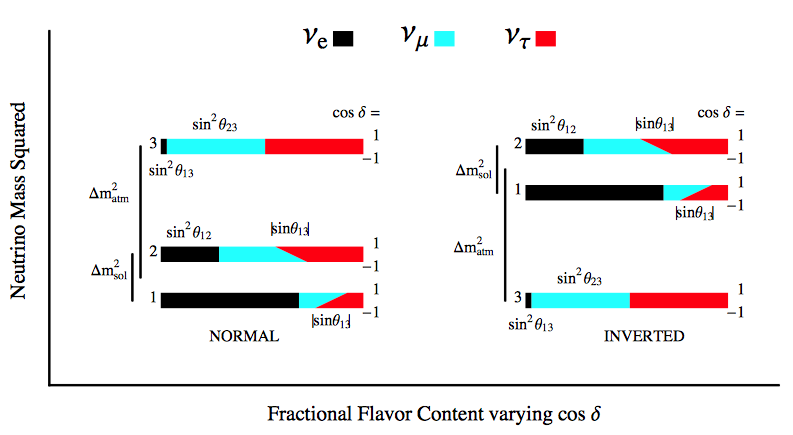
\includegraphics[width=\textwidth]{figures/MassSplitting.png}
  \caption[Neutrino Mass Splitting Schematic]{A schematic of the mass splittings between the three known neutrino mass states and how much they couple to each of the flavor states \cite{ref:MassSplitRef}.}
  \label{fig:MassSplit}
\end{figure}

Two oscillation probabilities that are of interest to \nova~are the muon neutrino survival probability and electron neutrino appearance from a muon neutrino beam. Since $\vert\dmxy{1}{2}\vert$ is so much smaller than $\vert\dmxy{2}{3}\vert$, the solar oscillation baseline is much longer, thus the oscillation probability is first dominated by terms containing $\dmxy{2}{3}$. This is the case for \nova. Furthermore, the probability can be simplified by making making the assumption that $\vert \dmxy{2}{3} \vert \approx \vert \dmxy{1}{3} \vert$. Under these conditions, the survival probability of muon neutrinos is calculated as follows:
\beqa
P(\numu \rightarrow \numu) & \approx & 1 - 4\Usqxy{\mu}{3} (\Usqxy{\mu}{1} + \Usqxy{\mu}{2}) \sin^2 \Delta_{32} \label{eq:3MuToMu1} \\
& \approx & 1 - 4 s^2_{23} (1 - s^2_{13}) (c^2_{23} + s^2_{23} s^2_{13}) \sin^2 \Delta_{32} \label{eq:3MuToMu2} \\
& \approx & 1 - 4 s^2_{23} c^2_{23} \sin^2 \Delta_{32} + 4 s^2_{23} s^2_{13} (c^2_{23} - s^2_{23}) \sin^2 \Delta_{32} \label{eq:3MuToMu3} \\
& = & 1 - \sin^2 2\thxy{2}{3} \sin^2 \Delta_{32} + 4 \sin^2 \thxy{2}{3} \sin^2 \thxy{1}{3} \cos^2 2\thxy{2}{3} \sin^2 \Delta_{32} \quad\quad
\label{eq:3MuToMu}
\eeqa

\n Between equations \ref{eq:3MuToMu2} and \ref{eq:3MuToMu3}, the term proportional to $s^4_{13}$ was dropped using the current knowledge that $s^2_{13}$ is small \cite{ref:PDG}. Note that if $\theta_{13}$ were $0$, then equation \ref{eq:3MuToMu} would reduce to equation \ref{eq:2NuSurv}, the two neutrino survival probability.

The full $3$ flavor electron neutrino appearance from muon neutrino oscillation probability is often written in the form \cite{ref:ThesisEvan}:
\beq
P(\nuanu_{\mu} \rightarrow\,\nuanu_{e}) = P_{atm} + 2\sqrt{P_{atm}}\sqrt{P_{sol}} \left(\cos\delta \cos\Delta_{32}\, \varmp\, \sin\delta \sin\Delta_{32} \right) + P_{sol}
\label{eq:3MuToE}
\eeq

\n where
\beqa
\sqrt{P_{atm}} & \equiv & \sin \thxy{2}{3} \sin 2\thxy{1}{3} \sin \Delta_{32} \label{eq:Patm} \\
\sqrt{P_{sol}} & \equiv & \cos \thxy{2}{3} \sin 2\thxy{1}{2} \sin \Delta_{21} \label{eq:Psol}
\eeqa

\n where the approximation $\vert \dmxy{2}{3} \vert \approx \vert \dmxy{1}{3} \vert$ has been made and higher order terms of $s^2_{13}$ been dropped. For an experiment at a short enough baseline such as \nova, the $P_{sol}$ term is negligible as it depends on a higher order term of the solar mass splitting. The cross term is also not the dominant effect as it also depends upon the solar mass splitting, but it demonstrates interesting behavior. The $\cos\delta$ term is $CP$ conserving, but the $\sin\delta$ term exhibits $CP$ violation. This is why $\delta$ is called the $CP$ violating phase angle.

\section{Matter Effects}
\label{sec:TheoryMatter}

So far, the oscillation formalism has been developed only considering neutrinos in a vacuum. However, most neutrino oscillation experiments involve neutrinos traveling through matter, be it the Sun or the Earth. This affects the oscillation probabilities in a process called the Mikheyev-Smirnov-Wolfenstein effect, or MSW effect. The phenomenon was first proposed by Wolfenstein in $1978$ \cite{ref:Wolfenstein}; Mikheyev and Smirnov built upon that work in $1985$ \cite{ref:MSW} as a possible solution for the solar neutrino problem.

\begin{figure}[t]
  \begin{center} $
  \begin{array}{c c}
    {
    \begin{fmffile}{MSWnue}
      \begin{fmfgraph*}(150,120)
        \fmfleft{n1,l2}
        \fmfright{l1,n2}
        \fmf{fermion}{n1,v1,l1}
        \fmf{fermion}{l2,v2,n2}
        \fmf{photon, tension=.75, label=$W^-$}{v1,v2}
        \fmflabel{$\nue$}{n1}
        \fmflabel{$e$}{l1}
        \fmflabel{$\nue$}{n2}
        \fmflabel{$e$}{l2}
      \end{fmfgraph*}
    \end{fmffile}
    }
    \quad \quad & \quad \quad
    {
    \begin{fmffile}{MSWanue}
      \begin{fmfgraph*}(150,120)
        \fmfleft{n1,l1}
        \fmfright{n2,l2}
        \fmf{fermion}{l1,v1,n1}
        \fmf{fermion}{n2,v2,l2}
        \fmf{photon, tension=.75, label=$W^-$}{v1,v2}
        \fmflabel{$\nue$}{n1}
        \fmflabel{$e$}{l1}
        \fmflabel{$\nue$}{n2}
        \fmflabel{$e$}{l2}
      \end{fmfgraph*}
    \end{fmffile}
    }
  \end{array} $
  \vspace{3 mm}
  \caption[MSW Effect Interactions]{CC coherent forward scattering interactions involved in the MSW effect. Left: Scattering of electron neutrinos on electrons. Right: Scattering of anti-electron neutrinos on electrons.}
  \label{fig:MSW}
  \end{center}
\end{figure}

The MSW effect is the CC coherent forward scattering of neutrinos off of the electrons in ordinary matter, a channel only available to electron flavor neutrinos and anti-neutrinos. Figure \ref{fig:MSW} illustrates the interactions. The electrons contribute an additional potential term, $V_e = \pm \sqrt{2}G_F N_e$, where $G_F$ is Fermi's constant, $N_e$ is the electron number density, the positive sign is for neutrinos, and the negative for anti-neutrinos. Neutrinos also forward scatter off the neutrons and protons in matter via neutral current interactions, but this only provides an overall phase as all neutrino flavors participate in these interactions equally. The matter induced potential adds an additional term to the Schr\"{o}dinger equation, affecting the time evolution of the flavor states and thus changing the oscillation probabilities.

The following derivation will consider the MSW effect in the case of two neutrino flavors. The time evolution of the flavor states is written as follows:
\beq
i \begin{pmatrix} \nue \\ \numu \end{pmatrix} = \left[ U \begin{pmatrix} \frac{m^2_1}{2E} & 0 \\ 0 & \frac{m^2_2}{2E} \end{pmatrix} U^\dagger + \begin{pmatrix} \pm V_e & 0 \\ 0 & 0 \end{pmatrix} \right] \begin{pmatrix} \nue \\ \numu \end{pmatrix}
\label{eq:2NuSchro}
\eeq

\n Inserting the 2 flavor PMNS matrix from equation \ref{eq:2NuU}, applying some trigonometric identites, and dropping common diagonal terms, equation \ref{eq:2NuSchro} simplifies to
\beq
i \begin{pmatrix} \nue \\ \numu \end{pmatrix} = \frac{1}{4E} \begin{pmatrix} -\dmxy{1}{2} \cos 2\theta \pm 4E V_e & \dmxy{1}{2} \sin 2\theta \\ \dmxy{1}{2} \sin 2\theta & \dmxy{1}{2} \cos 2\theta \end{pmatrix} \begin{pmatrix} \nue \\ \numu \end{pmatrix}.
\label{eq:2NuSchroNoDiag}
\eeq

\n The diagonal terms are dropped because they can be absorbed by the phase convention of the neutrino states. This Hamiltonian can be re-diagonalized with another unitary transformation, $H_{M} = U_{M}^\dagger H U_{M}$, with the following results:
\beqa
H_{M} & = & \frac{1}{2} \begin{pmatrix} -\frac{\Delta m^2_{M}}{2E} & 0 \\ 0 & \frac{\Delta m^2_{M}}{2E} \end{pmatrix} \label{eq:HMSW} \\
U_{M} & = & \begin{pmatrix} \cos \theta_{M} & \sin \theta_{M} \\ -\sin \theta_{M} & \cos\theta_{M} \end{pmatrix}, \label{eq:UMSW}
\eeqa

\n where
\beqa
\sin 2\theta_{M} & \equiv & \frac{\sin 2\theta}{A_{M}} \label{eq:thetaMSW} \\
\Delta m^2_{M} & \equiv & \dmxy{1}{2} A_{M} \label{eq:msqMSW} \\
A_{M} & \equiv & \sqrt{ \left( \cos 2\theta \mp \frac{2EV_e}{\dmxy{1}{2}} \right)^2 + \sin^2 2\theta } \label{eq:AMSW},
\eeqa

\n and now the negative sign in $A_M$ is for neutrinos and the positive sign for anti-neutrinos. As the electron number density goes to $0$, so too does $V_e$ and the vacuum solution is recovered.

From the form of this solution, it can be seen that the Hamiltonian takes the same form as that in vacuum oscillations, but with modified effective masses. Likewise, $U_M$ has the same form as the $2$ neutrino PMNS matrix, so $\theta_M$ can be considered the effective mixing angle. In the absence of neutrino oscillations (when $\theta = 0$), matter effects cannot ``create'' them. However, even for small angles $\theta$, the matter effect can create a resonant effect pushing the effective mixing angle, $\theta_M$, maximally to $45^\circ$. This occurs when the term in parenthesis in the definition of $A_M$ is $0$ (equation \ref{eq:AMSW}).
\beq
N_e^{res} = \frac{\dmxy{1}{2} \cos 2\theta}{2\sqrt{2} G_F E}
\label{eq:MSWres}
\eeq

In the case of $3$ neutrinos, the same procedure is followed to diagonalize the Hamilton and obtain effective values for the various oscillation parameters. The effects are considerably more complicated, but the general effect is the same--matter changes the effective neutrino mass and alters the oscillation probability curves differently for neutrinos and anti-neutrinos. Under the same conditions that were used to calculate $P(\nuanu_\mu \rightarrow \nuanu_e)$ in section \ref{sec:Theory3}, the results can be simplified to a few basic replacements \cite{ref:3NuMatter}.
\beq
P(\nuanu_{\mu} \rightarrow\,\nuanu_{e}) = P^M_{atm} + 2\sqrt{P^M_{atm}}\sqrt{P^M_{sol}} \left(\cos\delta \cos\Delta_{32}\, \varmp\, \sin\delta \sin\Delta_{32} \right) + P^M_{sol}
\label{eq:3MuToEMSW}
\eeq

\n This is exactly the same form as equation \ref{eq:3MuToE}. The interesting effects are seen with how $P^M_{atm}$ and $P^M_{sol}$ differ from their respective vacuum counterparts.
\beqa
\sqrt{P^M_{atm}} & \equiv & \sin \thxy{2}{3} \sin 2\thxy{1}{3} \frac{\sin (\Delta_{31} - aL)}{\Delta_{31} - aL} \Delta_{31} \label{eq:PatmMSW} \\
\sqrt{P_{sol}} & \equiv & \cos \thxy{2}{3} \sin 2\thxy{1}{2} \frac{\sin(aL)}{aL} \Delta_{21} \label{eq:PsolMSW}
\eeqa

\n Here, $a \equiv \pm G_F N_e / \sqrt{2}$ where the positive sign is for neutrinos and the negative sign for anti-neutrinos. For the Earth, $\vert a \vert \approx 1/3500\unit{km}$.

The combined effect that appears in equations \ref{eq:3MuToEMSW}, \ref{eq:PatmMSW}, and \ref{eq:PsolMSW} due to the presence of matter plays an interesting role in the search for CP violation. The MSW effect by itself mimics CP violation as it alters oscillation probabilities for neutrinos and anti-neutrinos differently. Depending on the value of $\delta$ that nature has chosen, the differences in oscillation probabilities due to the CP violation angle and the MSW effect can either compound or cancel out.

\section{Current Measurements}
\label{sec:BestMeasures}

Most of the free parameters in the PMNS matrix have been measured by various solar, atmospheric, accelerator, and reactor neutrino experiments. However, any given neutrino experiment does not have sensitivity to all of the oscillation parameters. Instead, experiments are sensitive to specific angles based on their baseline and the energies of the neutrinos they observe. Solar neutrino experiments, such as GALLEX, SAGE, Super-K, and SNO, measure neutrinos with energies on the order of several MeV after a very long baseline, and are most sensitive to $\theta_{12}$ and $\dmxy{1}{2}$. Due to the strong MSW effect within the Sun, solar neutrino experiments also determined the ordering of mass states $\nu_1$ and $\nu_2$; $\nu_2$ is defined as the heavier state. Atmospheric neutrino experiments, such as Super-K, SNO, and MINOS, measure neutrinos generated by cosmic ray collisions with the Earth's atmosphere, and are sensitive to $\theta_{23}$ and $\dmxy{2}{3}$.

Reactor neutrino experiments, such as Chooz, Double Chooz, RENO, and Daya Bay, measure $\anue$ generated by nearby nuclear reactors. Like solar neutrinos, reactor neutrinos have energies on the order of a few MeV. By measuring these neutrinos with a short baseline ($O(1 km)$), the $2$ neutrino approximation is valid, so the oscillation probability can be approximated as:
\beq
P(\anue \rightarrow \anue) \approx 1 - \sin^2 2\theta_{13} \sin^2 \Delta_{31}.
\label{eq:2NuReactor}
\eeq

\n Daya Bay made the first nonzero measurement of $\theta_{13}$ in $2012$, reporting a value of $\sin^2 2\theta_{13} = 0.092 \pm 0.016\mbox{ (stat)} \pm 0.005\mbox{ (syst)}$ after taking just $55$ days of data \cite{ref:DayaBay2012}. This result excluded a zero value for $\theta_{13}$ at $5.2\sigma$ and is shown in figure \ref{fig:DayaBay2012}. Since that result, the limits have only continued to improve, and the leading measurement still comes from Daya Bay.

\begin{figure}[!htb]
  \centering
  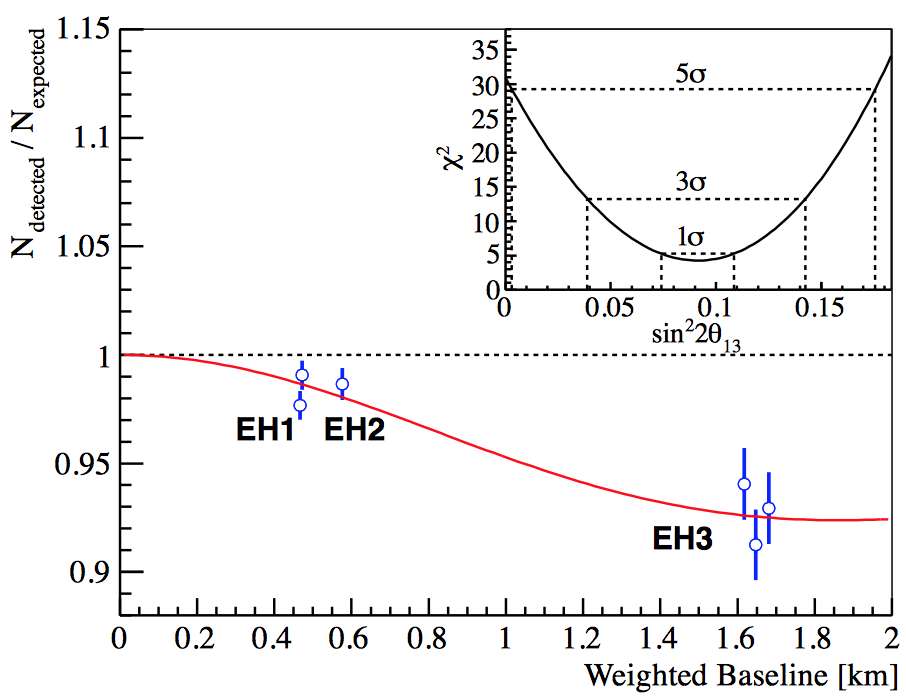
\includegraphics[width=0.75\textwidth]{figures/DayaBay2012.png}
  \caption[First Measurement of $\theta_{13}$ from Daya Bay]{First measurement of $\theta_{13}$ from Daya Bay \cite{ref:DayaBay2012}. The points show the ratio of observed to expected events assuming $\theta_{13} = 0$. Each point is a measurement at a different detector. The inset in the upper corner shows the $\chi^2$ value vs value of $\sin^2 2\theta_{13}$, and excludes $\theta_{13} = 0$ at greater than $5\sigma$.}
  \label{fig:DayaBay2012}
\end{figure}

Accelerator neutrino experiments, such as MINOS, T2K, and \nova, begin with a beam of nearly pure $\nuanu_\mu$ and search for both a disappearance of $\nuanu_\mu$ and appearance of other neutrino flavors. These experiments are sensitive to $\theta_{13}$, $\theta_{23}$, $\dmxy{2}{3}$, and $\delta$. The experiments that have the largest matter effect are the most sensitive to $\delta$ and the mass hierarchy.

Global fits to the combined data of these (and other) neutrino experiments have been performed and summarized in \cite{ref:PDG, ref:BestFits3}; the best fit values are shown in table \ref{tab:BestFits3}. While most of the parameters have been measured with good precision, there are still a few lingering questions. From the table it is clear that a much better measurement on the CP violation angle is needed. The mass hierarchy still needs to be definitively measured as well. The other main question is whether $\theta_{23}$ is maximal, and if not, whether it is in the lower or upper octant.
\begin{table}[!htb]
  \begin{center}
    \begin{tabular}{l c l l}
      \hline\hline
      \multicolumn{2}{c}{Parameter} & \multicolumn{1}{c}{Best-Fit $(\pm 1\sigma)$} & \multicolumn{1}{c}{$3\sigma$ Range} \\
      \hline
      $\dmxy{1}{2} \left[10^{-5}\evsq\right]$ && $7.54^{+0.26}_{-0.22}$ & $6.99 - 8.18$ \\
      \multirow{2}{*}{$\vert \Delta m^2 \vert \left[10^{-3}\evsq\right]$} & NH & $2.43 \pm 0.06$ & $2.23 - 2.61$ \\
      & IH & $2.38 \pm 0.06$ & $2.19 - 2.56$ \\
      $\sin^2 \theta_{12}$ && $0.308 \pm 0.017$ & $0.259 - 0.359$ \\
      \multirow{2}{*}{$\sin^2 \theta_{23}$} & NH & $0.437^{+0.033}_{-0.023}$ & $0.374 - 0.628$ \\
      & IH & $0.455^{+0.039}_{0.031}$ & $0.380 - 0.641$ \\
      \multirow{2}{*}{$\sin^2 \theta_{13}$} & NH & $0.0234^{+0.0020}_{-0.0019}$ & $0.0176 - 0.0295$ \\
      & IH & $0.0240^{+0.0019}_{-0.0022}$ & $0.0178 - 0.0298$ \\
      \multirow{2}{*}{$\delta/\pi$ ($2\sigma$ range)} & NH & $1.39^{+0.38}_{-0.27}$ & $(0.00 - 0.16) \oplus (0.86 - 2.00)$ \\
      & IH & $1.31^{+0.29}_{-0.33}$ & $(0.00 - 0.02) \oplus (0.70 - 2.00)$\\
      \hline
    \end{tabular}
    \caption[Best Fit Parameters for Three Neutrino Oscillation Model]{Current status of best fit oscillation parameters, from \cite{ref:PDG, ref:BestFits3}. The last column shows the allowed values within a $3\sigma$ range, with the exception of $\delta$, which is shown at a $2\sigma$ range. This is because the current global best fit for $\delta$ still allows the full range from $0$ to $2\pi$ at $3\sigma$. \nova~should vastly improve the limits on $\delta$.}
    \label{tab:BestFits3}
  \end{center}
\end{table}

Current and next generation reactor experiments have a great outlook to answer these outstanding questions. Making use of the MSW effect, the $\nue$ and $\anue$ appearance results from experiments like T2K and \nova~could simultaneously measure $\delta$, the mass hierarchy, and $\theta_{23}$ octant. The prospects for \nova~to make these measurements are shown in figure \ref{fig:BiProb}. The first analysis results from \nova~\cite{ref:NOvAFANuE, ref:NOvAFANuMu} were published after taking about $10\%$ of the experiments design statistics and already show promise. The \nova~measurement for $\delta$, shown in figure \ref{fig:NOvAFADelta}, provide a hint toward the normal hierarchy and eliminate portions of $\delta$ space at $90\%$ confidence.

\begin{figure}[!htb]
  \centering
  \begin{subfigure}{.48\textwidth}
    \centering
    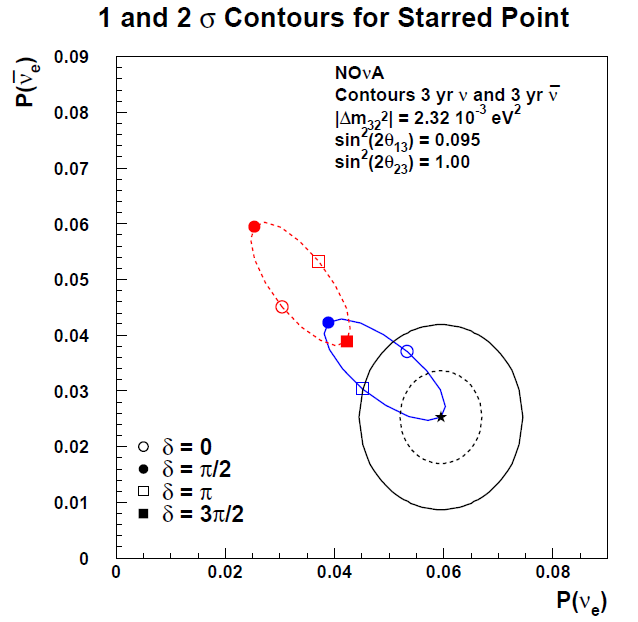
\includegraphics[width=1\linewidth]{figures/BiProbability.png}
  \end{subfigure}
  \begin{subfigure}{.48\textwidth}
    \centering
    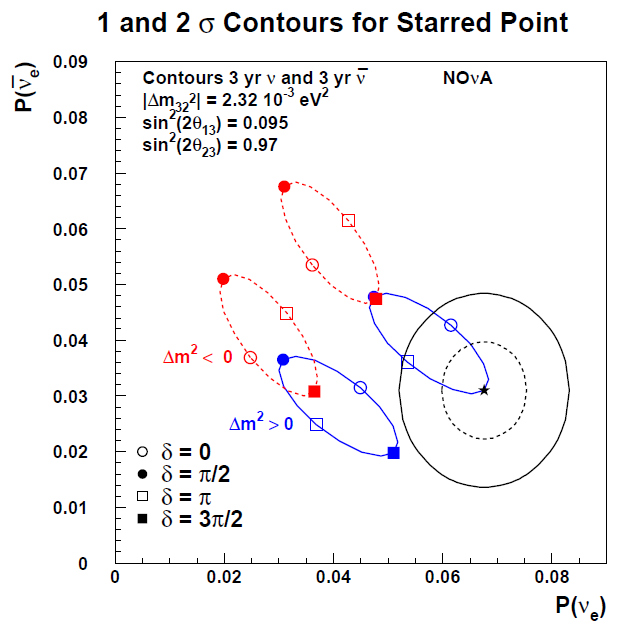
\includegraphics[width=1\linewidth]{figures/BiProbabilityVary23.png}
  \end{subfigure}
  \caption[Bi-Probability Plots for $\nue$ Appearance]{Probability of $\nue$ appearance versus $\anue$ appearance at \nova. The blue ellipses are for the normal hierarchy; the red ellipses are for the inverted hierarchy. The starred points show a possible measurement \nova~could make. The matter effect can either constructively or destructively combine with the CP violation effect. A larger matter effect, further separates the two mass hierarchy ellipses. This corresponds to neutrinos passing through more matter. On the left, $\theta_{23}$ is assumed to be $45^\circ$ for maximal mixing, purely showcasing the interference between the matter and CP violation effects. On the right, $\theta_{23}$ is non-maximal, showing how the dependence on $\theta_{23}$ affects both ellipses in the same way.}
  \label{fig:BiProb}
\end{figure}

\begin{figure}[!htb]
  \centering
  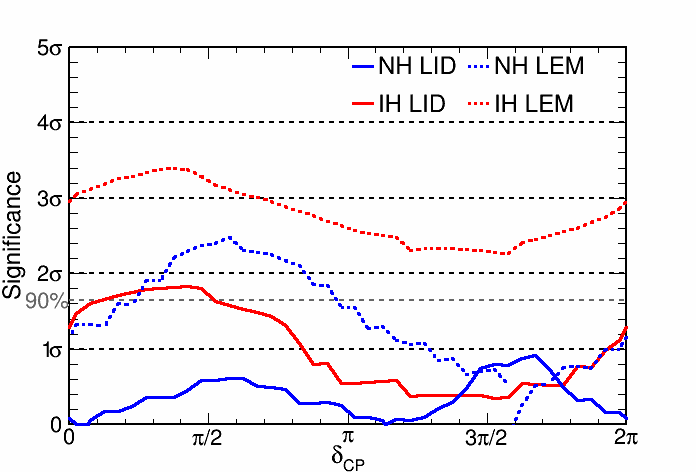
\includegraphics[width=0.75\textwidth]{figures/NOvAFADelta.png}
  \caption[First Measurement of $\delta$ by \nova]{First measurement of $\delta$ from \nova~\cite{ref:NOvAFANuE}. The plot shows the significance of the difference between the observed and predicted number of events as a function of delta. \nova~used a primary and secondary selection technique, the primary (secondary) technique is shown as the solid (dotted) line. The secondary selection disfavors the inverted hierarchy for all values of $\delta$.}
  \label{fig:NOvAFADelta}
\end{figure}

\section{Sterile Neutrinos}
\label{sec:Theory3+1}

The analysis presented in this dissertation considers sterile neutrinos in a $3 + 1$ model. This adds a fourth neutrino flavor state, $\nu_s$, and mass state, $\nu_4$, and the PMNS matrix becomes a $4\times4$ matrix. Given that standard three flavor oscillations explain solar, atmospheric, and long-baseline oscillations so well, this fourth state must be mostly sterile, i.e., $\vert \Uxy{\alpha}{4} \vert \ll 1$ for $\alpha \in \{e, \mu, \tau\}$.

The experimental evidence discussed in section \ref{sec:SterHist} suggests a mass splitting of $\Delta m^2 \sim O(1\unit{eV}^2)$. If the fourth neutrino mass state were the lightest, then all of the other mass states would have absolute masses $m \gtrsim 1\unit{eV}$. However, the sum of the active neutrino masses is well constrained by cosmology; the most recent Planck results reported $\sum m_\nu < 0.23\unit{eV}$ \cite{ref:Planck}. Consequently, it is assumed that the additional neutrino mass state is heavier than the other three. Furthermore, since $\dmxy{i}{4} \gg \vert \dmxy{i}{j} \vert$ for $i, j < 4$, it is assumed that $\Delta_{41} \approx \Delta_{42} \approx \Delta_{43}$.

As mentioned above, adding a fourth neutrino state expands the PMNS matrix into a $4\times4$ matrix. It can be written as the product of individual (complex) rotation matrices, as in the second line of equation \ref{eq:3NuU}. This adds an additional $3$ real rotation angles and $2$ complex phases. It is a matter of convention on how exactly to add these mixing angles into the PMNS matrix, but as physical results cannot be affected by a particular parametrization, it is best to choose the most convenient one. Following the parametrization in \cite{ref:GlobalFit}, $U$ takes the form:
\beq
U = R_{34} C_{24} R_{23} R_{14} C_{13} C_{12},
\label{eq:4NuU}
\eeq

\n where $R_{ij}$ is a real matrix parametrized by a single, real mixing angle, $\theta_{ij}$, and $C_{ij}$ is a complex matrix parametrized by a real mixing angle $\theta_{ij}$ and complex phase $\delta_{ij}$. This parametrization is convenient because as was the case in section \ref{sec:Theory3}, the solar mass scale $\Delta_{21}$ is negligible, thus mixing angles parametrized by $C_{12}$ drop out of the oscillation probabilities. Based on this, equation \ref{eq:4NuU} can be expanded in terms of the mixing angles:
\beq
U = \begin{bmatrix} U_{e1} & U_{e2} & c_{14} s_{13} e^{-i\delta_{13}} & s_{14} \\ U_{\mu1} & U_{\mu2} & -s_{14} s_{13} e^{-i\delta_{13}} s_{24} e^{-i\delta_{24}} + c_{13} s_{23} c_{24} & c_{14} s_{24} e^{-i\delta_{24}} \\ U_{\tau1} & U_{\tau2} & -s_{14} c_{24} s_{34} s_{13} e^{-i\delta_{13}} - c_{13} s_{23} s_{34} s_{24} e^{i\delta_{24}} + c_{13} c_{23} c_{34} & c_{14} c_{24} s_{34} \\ U_{s1} & U_{s2} & -s_{14} c_{24} c_{34} s_{13} e^{-i\delta_{13}} - c_{13} s_{23} c_{34} s_{24} e^{i\delta_{24}} - c_{13} c_{23} s_{34} & c_{14} c_{24} c_{34} \end{bmatrix}
\label{eq:4NuUExpand}
\eeq

\n Above, only the columns that appear in the oscillation probabilities have been expanded. Before using these expanded forms, however, it is useful to write the oscillation probability formulae in terms of the matrix elements first.

For \nova, which starts with a nearly pure $\numu$ beam, the two most important oscillation probabilities are the $\numu$ survival probability, $P(\numu \rightarrow \numu)$ and the probability that a $\numu$ will not oscillate to a sterile neutrino, $1 - P(\numu \rightarrow \nu_s)$. Starting with equations \ref{eq:nuSurv} and \ref{eq:nuOsc}, these probabilities are calculated as follows, using the unitarity of $U$ to remove elements found in its the first two columns.
\beqa
P(\numu \rightarrow \numu) \approx 1 & - & 4 \Usqxy{\mu}{4} ( \Usqxy{\mu}{1} + \Usqxy{\mu}{2} + \Usqxy{\mu}{3} ) \sin^2 \Delta_{41} \nonumber \\
& - & 4 \Usqxy{\mu}{3} ( \Usqxy{\mu}{1} + \Usqxy{\mu}{2} ) \sin^2 \Delta_{31} \nonumber \\
\approx 1 & - & 4 \Usqxy{\mu}{4} ( 1 - \Usqxy{\mu}{4} ) \sin^2 \Delta_{41} \nonumber \\
& - & 4 \Usqxy{\mu}{3} ( 1 - \Usqxy{\mu}{3} - \Usqxy{\mu}{4} ) \sin^2 \Delta_{31}
\label{eq:4MuToMu}
\eeqa

\beqa
1 - P(\numu \rightarrow \nu_s) = 1 & + & 4 \sum_{i > j} \Re ( \Uxy{\mu}{i} \Ustxy{s}{i} \Uxy{s}{j} \Ustxy{\mu}{j} ) \sin^2 \Delta_{ij} \nonumber \\
& - & 2\sum_{i > j} \Im ( \Uxy{\mu}{i} \Ustxy{s}{i} \Uxy{s}{j} \Ustxy{\mu}{j} ) \sin 2\Delta_{ij} \nonumber \\
\approx 1 & + & 4 \Re ( C_{41, 42, 43} ) \sin^2 \Delta_{41} + 4 \Re ( C_{31, 32} ) \sin^2 \Delta_{31} \nonumber \\
& - & 2\Im ( C_{41, 42, 43} ) \sin 2\Delta_{41} - 2 \Im ( C_{31, 32} ) \sin 2\Delta_{31}
\label{eq:4MuToSStart}
\eeqa

\n In equation \ref{eq:4MuToSStart}, $C_{41, 42,43}$ and $C_{31,32}$ are sums of products of PMNS matrix elements.
\beqa
C_{41, 42, 43} & = & \Uxy{\mu}{4} \Ustxy{s}{4} ( \Uxy{s}{1} \Ustxy{\mu}{1} + \Uxy{s}{2} \Ustxy{\mu}{2} + \Uxy{s}{3} \Ustxy{\mu}{3} ) \nonumber \\
& = & \Uxy{\mu}{4} \Ustxy{s}{4} ( - \Uxy{s}{4} \Ustxy{\mu}{4} ) \nonumber \\
& = & -\Usqxy{\mu}{4} \Usqxy{s}{4}
\label{eq:C414243}
\eeqa

\n Note that this term is real, thus the term with $\Im(C_{41,42,43})$ in equation \ref{eq:4MuToSStart} drops out.
\beqa
C_{31, 32} & = & \Uxy{\mu}{3} \Ustxy{s}{3} ( \Uxy{s}{1} \Ustxy{\mu}{1} + \Uxy{s}{2} \Ustxy{\mu}{2} ) \nonumber \\
& = & -\Uxy{\mu}{3} \Ustxy{s}{3} ( \Uxy{s}{4} \Ustxy{\mu}{4} + \Uxy{s}{3} \Ustxy{\mu}{3}) \nonumber \\
& = & -\Usqxy{\mu}{3} \Usqxy{s}{3} - \Uxy{\mu}{3} \Ustxy{\mu}{4} \Ustxy{s}{3} \Uxy{s}{4} \nonumber \\
& = & -\Usqxy{\mu}{3} \Usqxy{s}{3} - \Re (\Uxy{\mu}{3} \Ustxy{\mu}{4} \Ustxy{s}{3} \Uxy{s}{4} ) - i \Im(\Uxy{\mu}{3} \Ustxy{\mu}{4} \Ustxy{s}{3} \Uxy{s}{4} ) \nonumber \\
& = & -\Usqxy{\mu}{3} \Usqxy{s}{3} - \Re (\Ustxy{\mu}{3} \Uxy{\mu}{4} \Uxy{s}{3} \Ustxy{s}{4} ) + i \Im(\Ustxy{\mu}{3} \Uxy{\mu}{4} \Uxy{s}{3} \Ustxy{s}{4} )
\label{eq:C3132}
\eeqa

\n The last equality in \ref{eq:C3132} was done so that all terms in the oscillation probability are subtracted from $1$. Using these results, equation \ref{eq:4MuToSStart} becomes
\beqa
1 - P(\numu \rightarrow \nu_s) \approx 1 & - & 4 \Usqxy{\mu}{4} \Usqxy{s}{4} \sin^2 \Delta_{41} \nonumber \\
& - & 4( \Usqxy{\mu}{3} \Usqxy{s}{3} + \Re( \Ustxy{\mu}{3} \Uxy{\mu}{4} \Uxy{s}{3} \Ustxy{s}{4} ) ) \sin^2 \Delta_{31} \nonumber \\
& - & 2 \Im ( \Ustxy{\mu}{3} \Uxy{\mu}{4} \Uxy{s}{3} \Ustxy{s}{4} ) \sin 2\Delta_{31}.
\label{eq:4MuToS}
\eeqa

Equations \ref{eq:4MuToMu} and \ref{eq:4MuToS} are the probabilities that a $\numu$ will survive as a $\numu$ and survive as one of the active neutrino flavors, respectively. These can now be written in terms of the mixing angles. However, several approximations make the expressions much more bearable. First, based on the best value reported in section \ref{sec:BestMeasures}, the value of $s_{13}$ is taken as $0$. This has the fortunate side effect of removing any dependence on $\delta_{13}$ as well. Second, the value of $s_{14}$ is also taken as $0$, based on reactor and other constraints, e.g. \cite{ref:DayaSterile, ref:Th14Con}. Note that in the relevant matrix elements, $s_{13}$ and $s_{14}$ always appear together as a product, further justifying the approximation. The matrix element products that appear in the oscillation probabilities are calculated below.
\beqa
\Usqxy{\mu}{4} & = & s^2_{24} \label{eq:Usqmu4} \\
\Usqxy{s}{4} & = & c^2_{24} c^2_{34} \label{eq:Usqs4} \\
\Usqxy{\mu}{3} & = & s^2_{23} c^2_{24} \label{eq:Usqmu3} \\
\Usqxy{s}{3} & = & c^2_{23} s^2_{34} + s^2_{23} s^2_{24} c^2_{34} + 2c_{23} s_{23} s_{24} c_{34} s_{34} \cos \delta_{24} \label{eq:Usqs3} \\
\Ustxy{\mu}{3} \Uxy{\mu}{4} \Uxy{s}{3} \Ustxy{s}{4} & = & - s_{23} c^2_{24} s_{24} c_{34} (s_{23} s_{24} c_{34} + c_{23} s_{34} e^{-i\delta_{24}}) \label{eq:ReImUUUU} \\
\Re( \Ustxy{\mu}{3} \Uxy{\mu}{4} \Uxy{s}{3} \Ustxy{s}{4} ) & = & - s_{23} c^2_{24} s_{24} c_{34} (s_{23} s_{24} c_{34} + c_{23} s_{34} \cos \delta_{24}) \label{eq:ReUUUU} \\
\Im( \Ustxy{\mu}{3} \Uxy{\mu}{4} \Uxy{s}{3} \Ustxy{s}{4} ) & = & c_{23} s_{23} c^2_{24} s_{24} c_{34} s_{34} \sin \delta_{24} \label{eq:ImUUUU}
\eeqa

\n These results can be substituted into equations \ref{eq:4MuToMu} and \ref{eq:4MuToS}.
\beqa
P(\numu \rightarrow \numu) \approx 1 & - & 4 \Usqxy{\mu}{4} ( 1 - \Usqxy{\mu}{4} ) \sin^2 \Delta_{41} \nonumber \\
& - & 4 \Usqxy{\mu}{3} ( 1 - \Usqxy{\mu}{3} - \Usqxy{\mu}{4} ) \sin^2 \Delta_{31} \nonumber \\
\approx 1 & - & 4 s^2_{24} (1 - s^2_{24}) \sin^2 \Delta_{41} \nonumber \\
& - & 4 s^2_{23} c^2_{24} (1 - s^2_{23} c^2_{24} - s^2_{24}) \sin^2 \Delta_{31} \nonumber \\
\approx 1 & - & 4 c^2_{24} s^2_{24} \sin^2 \Delta_{41} - 4 c^4_{24} s^2_{23} (1 - s^2_{23}) \sin^2 \Delta_{31} \nonumber \\
\approx 1 & - & \sin^2 2\theta_{24} \sin^2 \Delta_{41} - c^4_{24} \sin^2 2\theta_{23} \sin^2 \Delta_{31}
\label{eq:4MuToMuAngles}
\eeqa

\beqa
1 - P(\numu \rightarrow \nu_s) \approx 1 & - & 4 \Usqxy{\mu}{4} \Usqxy{s}{4} \sin^2 \Delta_{41} \nonumber \\
& - & 4( \Usqxy{\mu}{3} \Usqxy{s}{3} + \Re( \Ustxy{\mu}{3} \Uxy{\mu}{4} \Uxy{s}{3} \Ustxy{s}{4} ) ) \sin^2 \Delta_{31} \nonumber \\
& - & 2 \Im ( \Ustxy{\mu}{3} \Uxy{\mu}{4} \Uxy{s}{3} \Ustxy{s}{4} ) \sin 2\Delta_{31} \nonumber \\
\approx 1 & - & 4 c^2_{24} s^2_{24} c^2_{34} \sin^2 \Delta_{41} \nonumber \\
& - & 4\left[ s^2_{23} c^2_{24} (c^2_{23} s^2_{34} + s^2_{23} s^2_{24} c^2_{34} + 2 c_{23} s_{23} s_{24}  c_{34} s_{34} \cos \delta_{24}) \right. \nonumber \\
&& \left. - s_{23} c^2_{24} s_{24} c_{34} ( s_{23} s_{24} c_{34} + c_{23} s_{34} \cos \delta_{24} ) \right] \sin^2 \Delta_{31} \nonumber \\
& - & 2 c_{23} s_{23} c^2_{24} s_{24} c_{34} s_{34} \sin \delta_{24} \sin 2\Delta_{31} \nonumber \\
\approx 1 & - & c^2_{34} \sin^2 2\theta_{24} \sin^2 \Delta_{41} \nonumber \\
& - & 4 \left[c^2_{23} s^2_{23} c^2_{24} s^2_{34} - s^2_{23} c^2_{24} s^2_{24} c^2_{34}(1 - s^2_{23}) \right. \nonumber \\
&& \left. + c_{23} s_{23} c^2_{24} s_{24} c_{34} s_{34} (2 s^2_{23} - 1) \cos \delta_{24} \right] \sin^2 \Delta_{31} \nonumber \\
& - & \frac{1}{4} c_{24} \sin 2\theta_{23} \sin 2\theta_{24} \sin 2\theta_{34} \sin \delta_{24} \sin 2\Delta_{31} \nonumber \\
\approx 1 & - & c^2_{34} \sin^2 2\theta_{24} \sin^2 \Delta_{41} - c^2_{24} (s^2_{34} - s^2_{24} c^2_{34}) \sin^2 2\theta_{23} \sin^2 \Delta_{31} \nonumber \\
& - & \frac{1}{4} c_{24} \sin 2\theta_{23} \sin 2\theta_{24} \sin 2\theta_{34} \sin \delta_{24} \sin 2\Delta_{31}
\label{eq:4MuToSAngles}
\eeqa

\n In the last equality, the term proportional to $\cos\delta_{24}$ was dropped noting that $2s^2_{23} - 1 \approx 0$. Even if it is not exact, there is already an additional factor of $s_{24} s_{34}$. Both $s_{24}$ and $s_{34}$ must be small in order to satisfy $\vert \Uxy{\mu}{4} \vert, \vert \Uxy{\tau}{4} \vert \ll 1$, thus the term proportional to $s_{24} s_{34} (2s^2_{23} - 1)$ can be considered higher order than the remaining terms.

The effect of each of the oscillation parameters can be seen in the figures below. Each page shows the $\numu$ survival probability followed by the active neutrino survival probability and uses the exact oscillation probabilities. Figures \ref{fig:LOverEDm41}-\ref{fig:LOverECP24} show how the mixing parameters that appear in equations \ref{eq:4MuToMuAngles} and \ref{eq:4MuToSAngles} affect the oscillation probabilities. Figures \ref{fig:LOverETh14}-\ref{fig:LOverECP13} are similar but show the much smaller effects of the parameters that dropped out of these equations due to approximations. (Solar mixing parameters are not shown.) The individual plots show different probabilities curves while varying a single oscillation parameter over a set of representative values; the mixing parameters that are not varied in a particular figure are held fixed to the values in table \ref{tab:LOverEValues}. In the figures, the bottom axis shows the neutrino $L/E$, thus the plots show oscillation probabilities at both the near and far detectors. The top axis shows the neutrino energy at each \nova detector, the dashed line separates the Near Detector (ND) on the left from the Far Detector (FD) on the right. Finally, the grey bands show the neutrino energies each detector is sensitive to; a darker color means a higher intensity of neutrinos at that energy.
\begin{table}[h]
  \begin{center}
    \begin{tabular}{c c}
      \hline\hline
      Oscillation Parameter & Value \\
      \hline
      $\rho$ & $2.84\unit{g/cm\textsuperscript{3}}$ \\
      $\Delta m^2_{21}$ & $7.53 \times 10^{-5}\evsq$ \\
      $\Delta m^2_{32}$ & $2.44 \times 10^{-3}\evsq$ \\
      $\Delta m^2_{41}$ & $0.5 \evsq$ \\
      $\sin^2 2\theta_{12}$ & $0.846$ \\
      $\sin^2 2\theta_{13}$ & $0.085$ \\
      $\theta_{23}$ & $\pi/4$ \\
      $\theta_{14}$ & $0$ \\
      $\theta_{24}$ & $10^\circ$ \\
      $\theta_{34}$ & $35^\circ$ \\
      $\delta_{13}$ & $0$ \\
      $\delta_{24}$ & $0$ \\
      \hline
    \end{tabular}
    \caption[Four Flavor Fixed Oscillation Parameters]{The $4$ flavor oscillation parameters assumed for studying the effects of different parameters on the oscillation probabilities.}
    \label{tab:LOverEValues}
  \end{center}
\end{table}

\begin{figure}[p]
  \centering
  \begin{tabular}{c}
    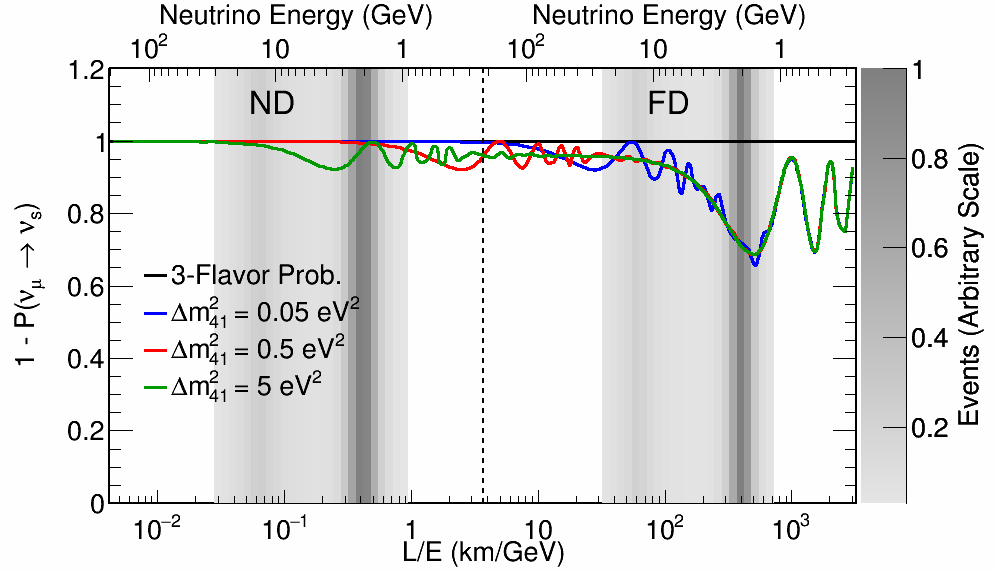
\includegraphics[width=0.95\textwidth]{figures/LOverE/LOverEMuSDm41.png} \\
    \\ \\
    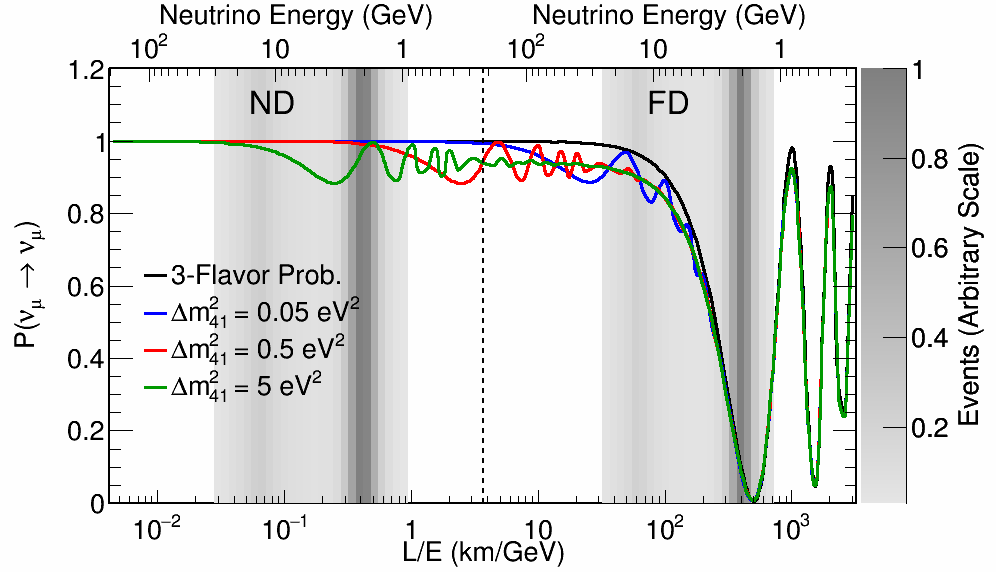
\includegraphics[width=0.95\textwidth]{figures/LOverE/LOverEMuMuDm41.png} \\
  \end{tabular}
  \caption[Oscillation Probabilities for Values of $\dmxy{1}{4}$]{Total active neutrino survival probability (top) and $\numu$ survival probability (bottom) for different values of $\dmxy{1}{4}$. Above $\dmxy{1}{4} = 0.5\unit{eV}^2$, oscillations start to affect the ND. The grey bands show the neutrino energy spectra observed by \nova, with darker colors representing a higher intensity of neutrinos. Parameters not varied in the figures are held fixed to values shown in table \ref{tab:LOverEValues}.}
  \label{fig:LOverEDm41}
\end{figure}

\begin{figure}[p]
  \centering
  \begin{tabular}{c}
    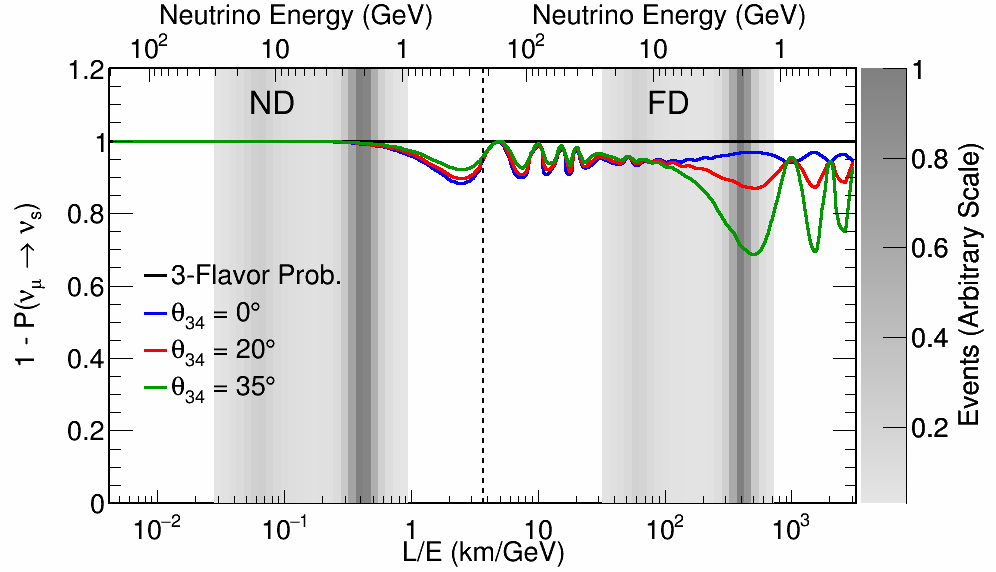
\includegraphics[width=0.95\textwidth]{figures/LOverE/LOverEMuSTh34.png} \\
    \\ \\
    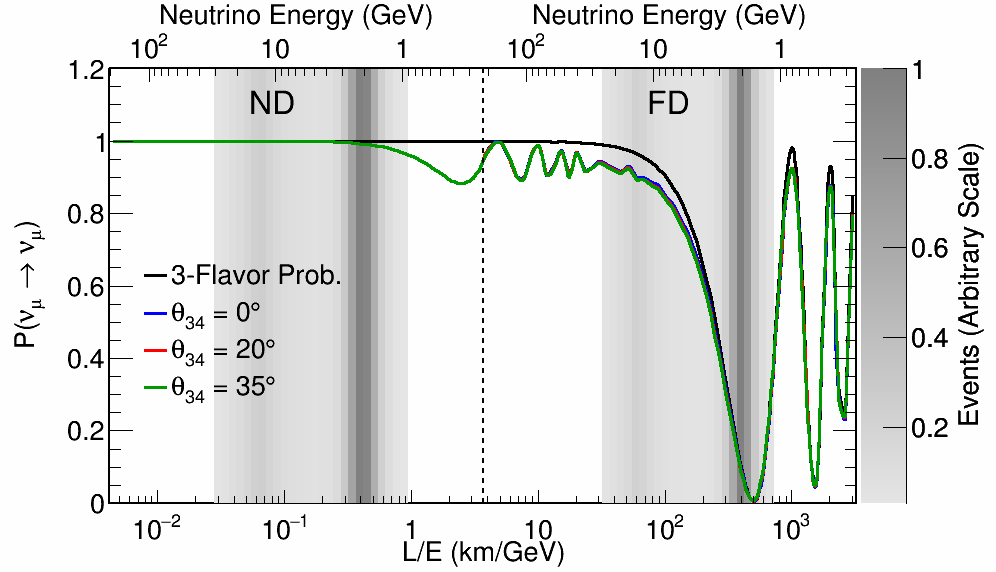
\includegraphics[width=0.95\textwidth]{figures/LOverE/LOverEMuMuTh34.png} \\
  \end{tabular}
  \caption[Oscillation Probabilities for Values of $\theta_{34}$]{Total active neutrino survival probability (top) and $\numu$ survival probability (bottom) for different values of $\theta_{34}$. The grey bands show the neutrino energy spectra observed by \nova, with darker colors representing a higher intensity of neutrinos. Parameters not varied in the figures are held fixed to values shown in table \ref{tab:LOverEValues}.}
  \label{fig:LOverETh34}
\end{figure}

\begin{figure}[p]
  \centering
  \begin{tabular}{c}
    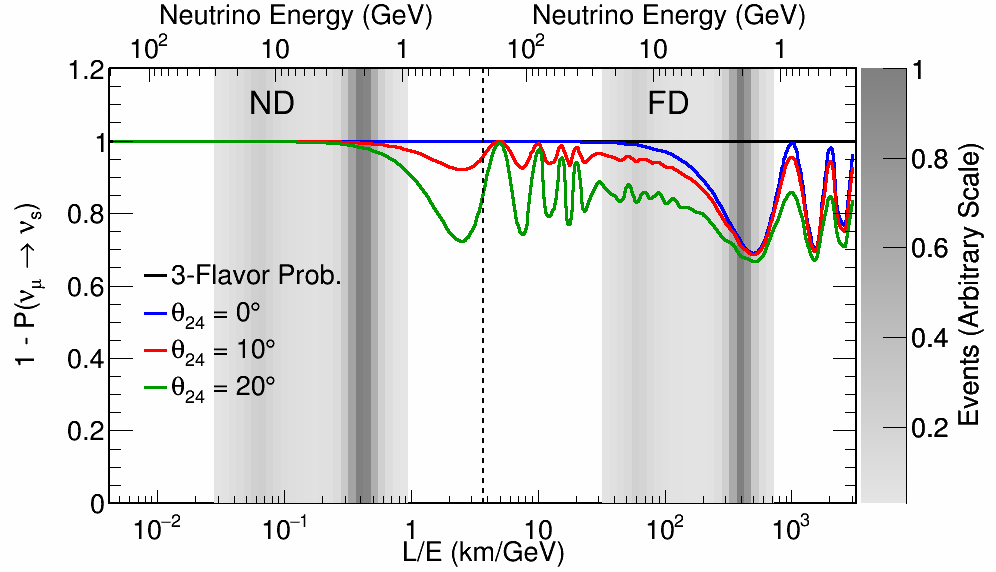
\includegraphics[width=0.95\textwidth]{figures/LOverE/LOverEMuSTh24.png} \\
    \\ \\
    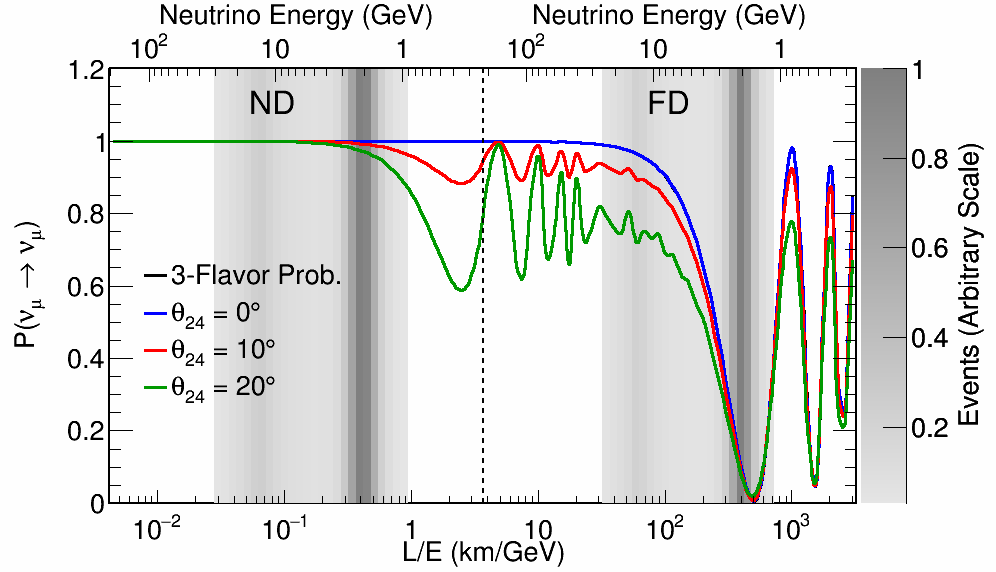
\includegraphics[width=0.95\textwidth]{figures/LOverE/LOverEMuMuTh24.png} \\
  \end{tabular}
  \caption[Oscillation Probabilities for Values of $\theta_{24}$]{Total active neutrino survival probability (top) and $\numu$ survival probability (bottom) for different values of $\theta_{24}$. The grey bands show the neutrino energy spectra observed by \nova, with darker colors representing a higher intensity of neutrinos. Parameters not varied in the figures are held fixed to values shown in table \ref{tab:LOverEValues}.}
  \label{fig:LOverETh24}
\end{figure}

\begin{figure}[p]
  \centering
  \begin{tabular}{c}
    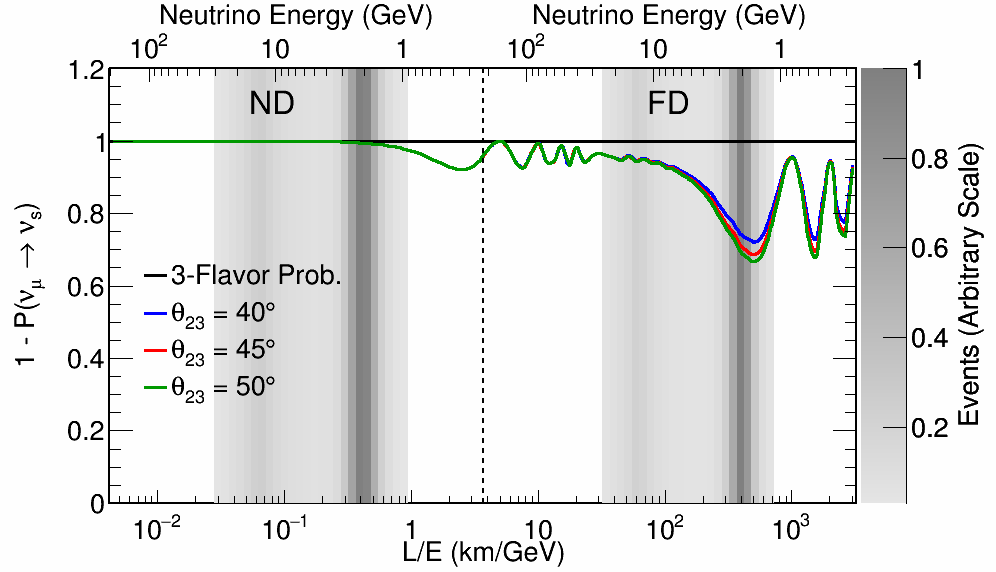
\includegraphics[width=0.95\textwidth]{figures/LOverE/LOverEMuSTh23.png} \\
    \\ \\
    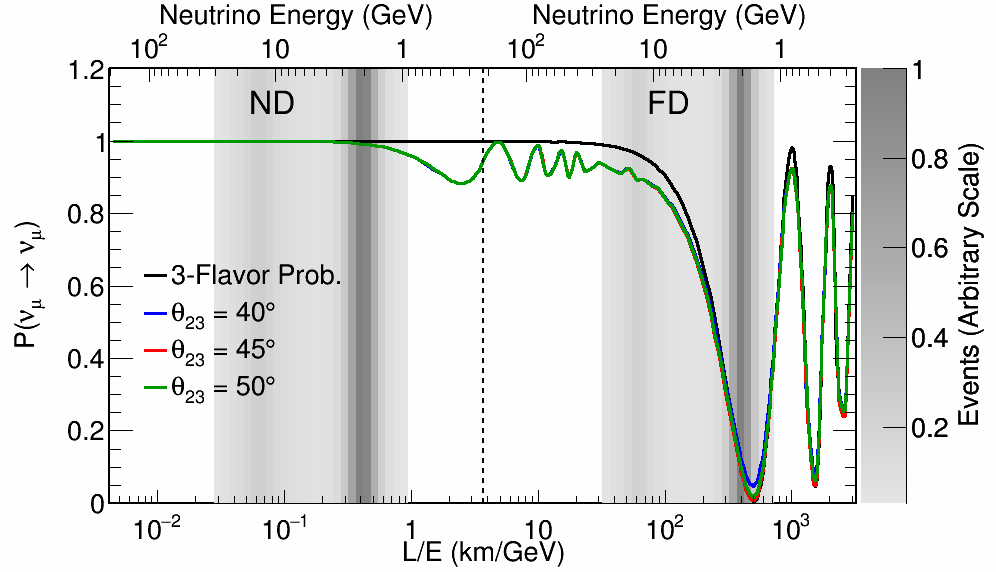
\includegraphics[width=0.95\textwidth]{figures/LOverE/LOverEMuMuTh23.png} \\
  \end{tabular}
  \caption[Oscillation Probabilities for Values of $\theta_{23}$]{Total active neutrino survival probability (top) and $\numu$ survival probability (bottom) for different values of $\theta_{23}$. Shifts in $\theta_{23}$ have a modest effect at the \nova~peak energy. The grey bands show the neutrino energy spectra observed by \nova, with darker colors representing a higher intensity of neutrinos. Parameters not varied in the figures are held fixed to values shown in table \ref{tab:LOverEValues}.}
  \label{fig:LOverETh23}
\end{figure}

\begin{figure}[p]
  \centering
  \begin{tabular}{c}
    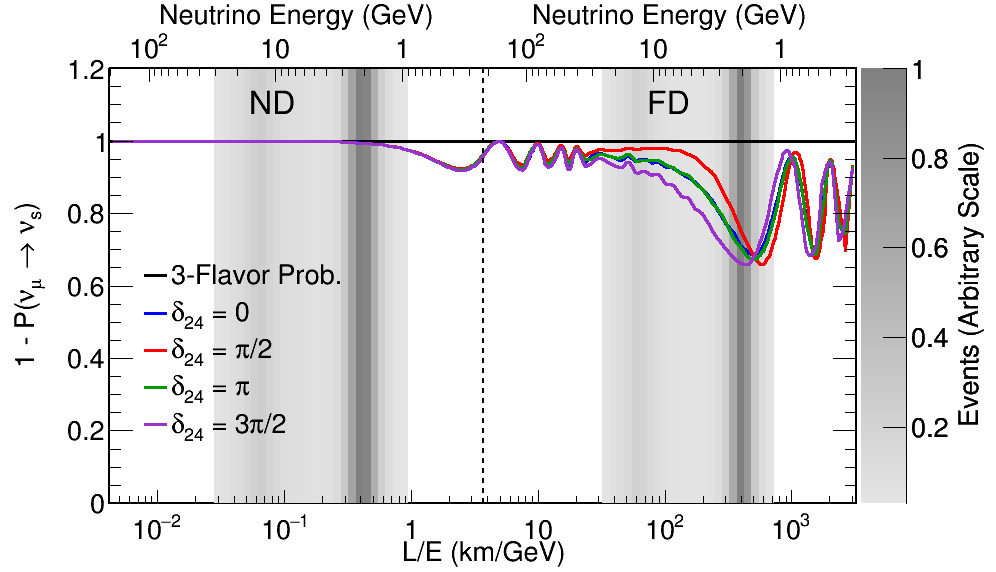
\includegraphics[width=0.95\textwidth]{figures/LOverE/LOverEMuSCP24.png} \\
    \\ \\
    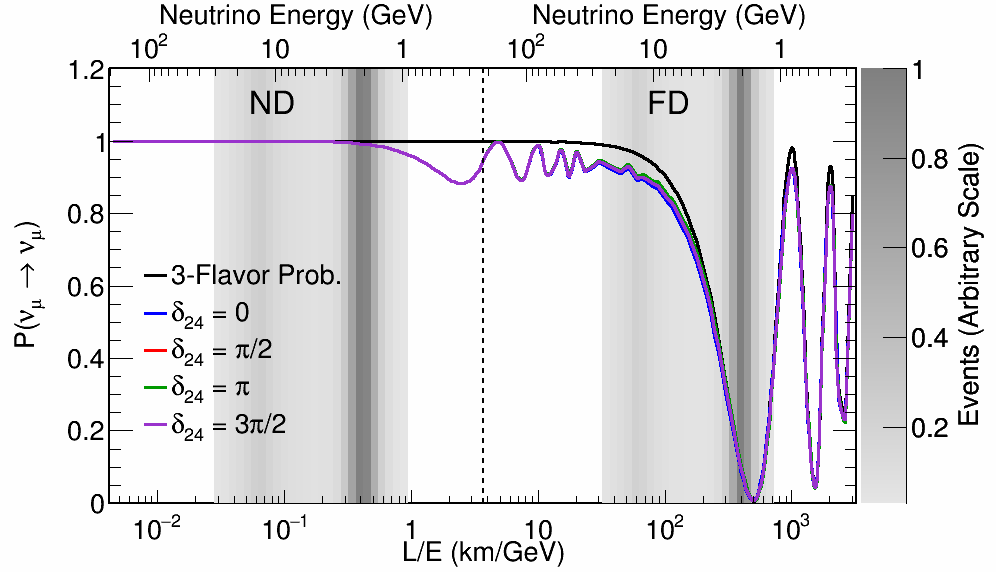
\includegraphics[width=0.95\textwidth]{figures/LOverE/LOverEMuMuCP24.png} \\
  \end{tabular}
  \caption[Oscillation Probabilities for Values of $\delta_{24}$]{Total active neutrino survival probability (top) and $\numu$ survival probability (bottom) for different values of $\delta_{24}$. The grey bands show the neutrino energy spectra observed by \nova, with darker colors representing a higher intensity of neutrinos. Parameters not varied in the figures are held fixed to values shown in table \ref{tab:LOverEValues}.}
  \label{fig:LOverECP24}
\end{figure}

\begin{figure}[p]
  \centering
  \begin{tabular}{c}
    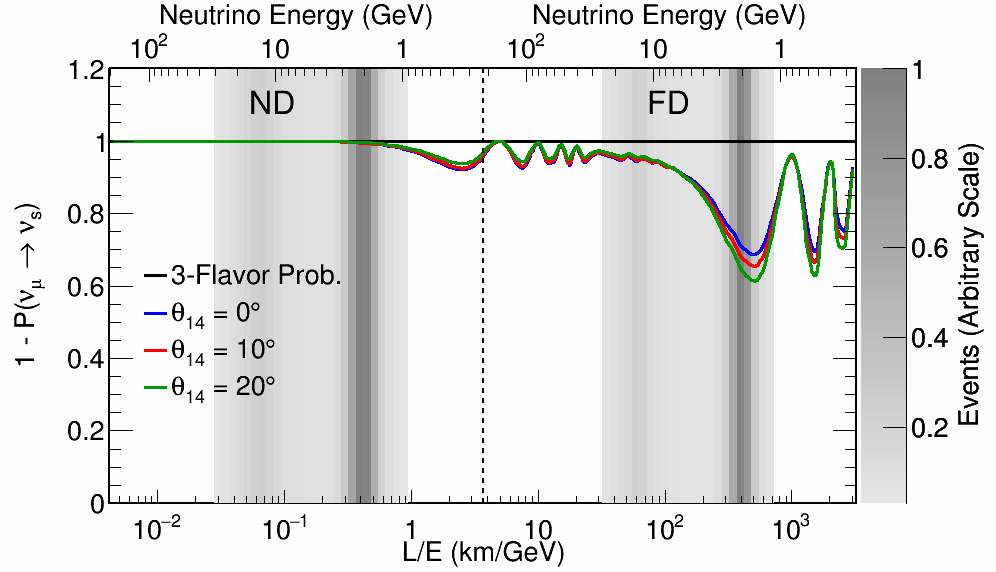
\includegraphics[width=0.95\textwidth]{figures/LOverE/LOverEMuSTh14.png} \\
    \\ \\
    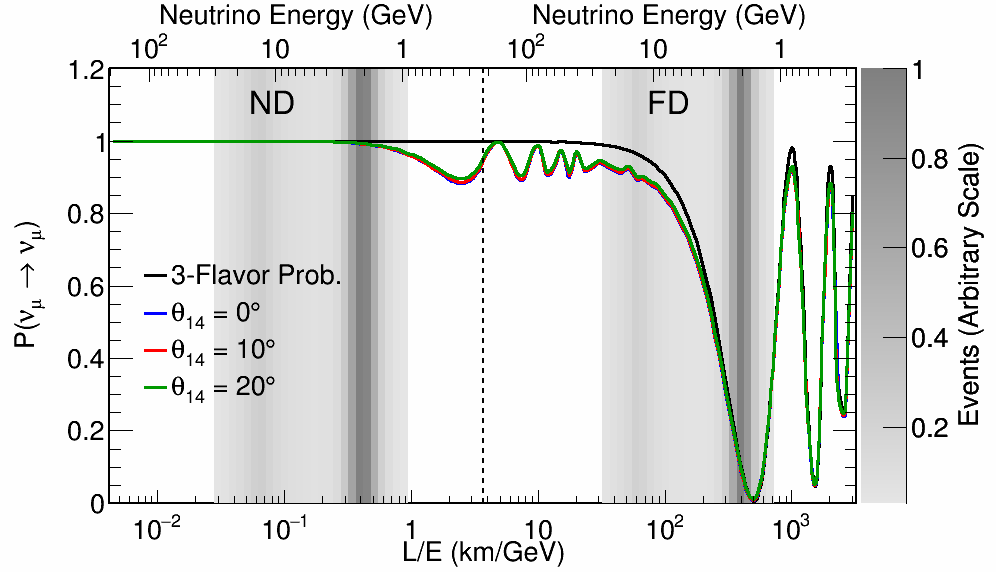
\includegraphics[width=0.95\textwidth]{figures/LOverE/LOverEMuMuTh14.png} \\
  \end{tabular}
  \caption[Oscillation Probabilities for Values of $\theta_{14}$]{Total active neutrino survival probability (top) and $\numu$ survival probability (bottom) for different values of $\theta_{14}$. The values shown are well outside of experimental bounds, but even these large shifts have only a small effect on the oscillation probabilities that is largely degenerate with $\theta_{23}$. The grey bands show the neutrino energy spectra observed by \nova, with darker colors representing a higher intensity of neutrinos. Parameters not varied in the figures are held fixed to values shown in table \ref{tab:LOverEValues}.}
  \label{fig:LOverETh14}
\end{figure}

\begin{figure}[p]
  \centering
  \begin{tabular}{c}
    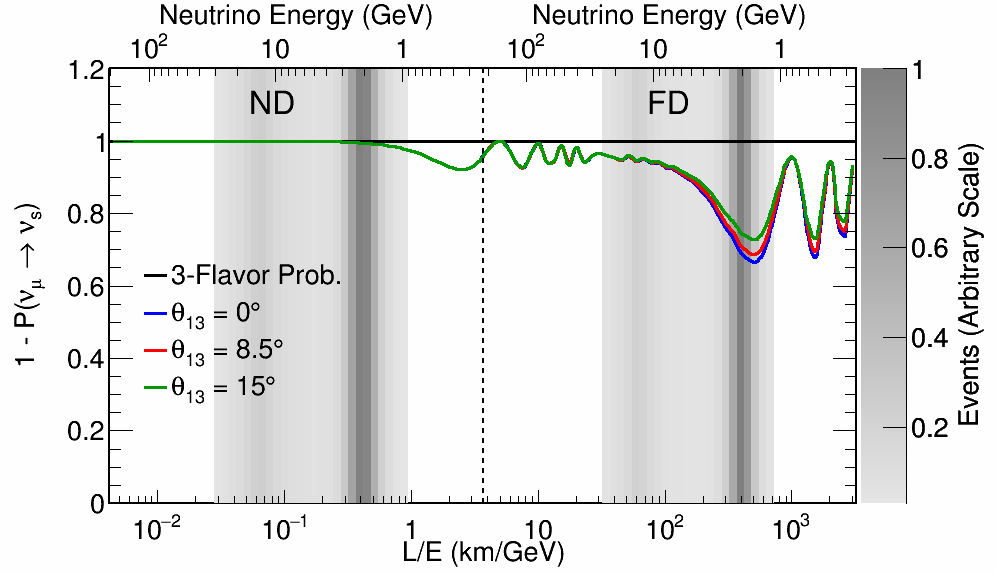
\includegraphics[width=0.95\textwidth]{figures/LOverE/LOverEMuSTh13.png} \\
    \\ \\
    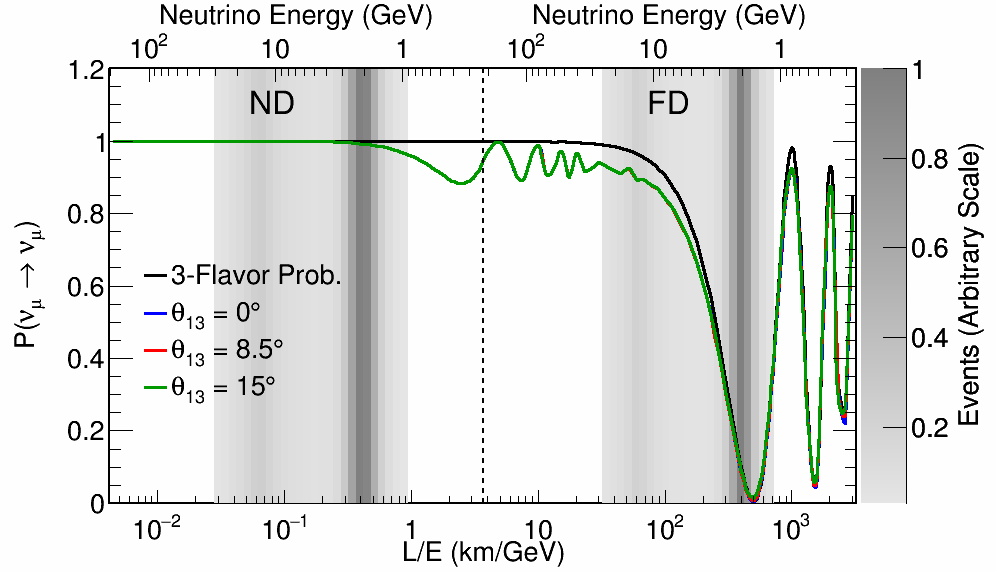
\includegraphics[width=0.95\textwidth]{figures/LOverE/LOverEMuMuTh13.png} \\
  \end{tabular}
  \caption[Oscillation Probabilities for Values of $\theta_{13}$]{Total active neutrino survival probability (top) and $\numu$ survival probability (bottom) for different values of $\theta_{13}$. The values shown are well outside of experimental bounds, but even these large shifts have only a small effect on the oscillation probabilities that is largely degenerate with $\theta_{23}$. The grey bands show the neutrino energy spectra observed by \nova, with darker colors representing a higher intensity of neutrinos. Parameters not varied in the figures are held fixed to values shown in table \ref{tab:LOverEValues}.}
  \label{fig:LOverETh13}
\end{figure}

\begin{figure}[p]
  \centering
  \begin{tabular}{c}
    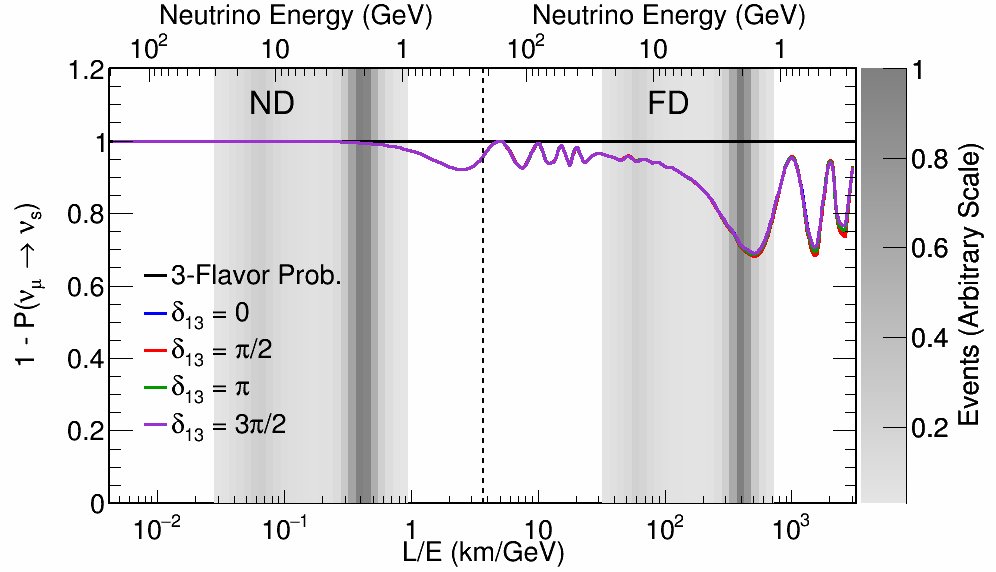
\includegraphics[width=0.95\textwidth]{figures/LOverE/LOverEMuSCP13.png} \\
    \\ \\
    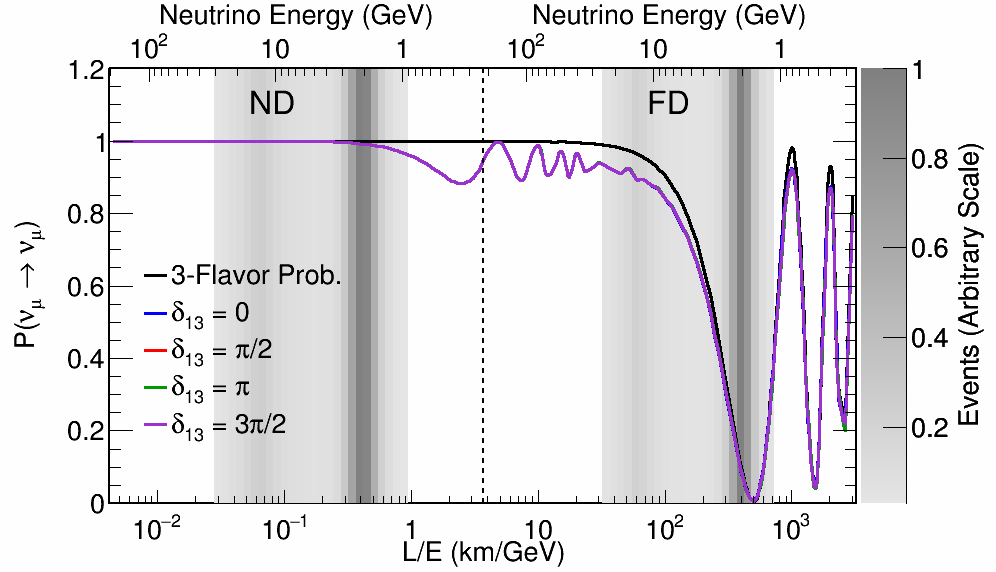
\includegraphics[width=0.95\textwidth]{figures/LOverE/LOverEMuMuCP13.png} \\
  \end{tabular}
  \caption[Oscillation Probabilities for Values of $\delta_{13}$]{Total active neutrino survival probability (top) and $\numu$ survival probability (bottom) for different values of $\delta_{13}$. The effects of $\delta_{13}$ are negligible on the oscillation probabilities. The grey bands show the neutrino energy spectra observed by \nova, with darker colors representing a higher intensity of neutrinos. Parameters not varied in the figures are held fixed to values shown in table \ref{tab:LOverEValues}.}
  \label{fig:LOverECP13}
\end{figure}

For the particular analysis presented in the rest of this dissertation, it is assumed that there are no Near Detector oscillations. Thus, the analysis will make measurements of $\theta_{24}$, $\theta_{34}$, and these will be translated into measurements of $\Usqxy{\mu}{4}$ and $\Usqxy{\tau}{4}$, and the results will be valid in the range $0.05 < \dmxy{1}{4} < 0.5\unit{eV}^2$.

To make the above measurements, the analysis presented here considers the rate of Neutral Current (NC) events. The rate of Charged Current (CC) events is obviously affected by neutrino oscillations. Given that standard three flavor oscillations already impact the number of CC events, it would be a difficult task to decouple oscillations between the active neutrino flavors and a fourth, sterile flavor. On the other hand, NC interactions are completely insensitive to the active neutrino flavors, and hence to oscillations between them. In the standard three flavor model, then, the total rate of NC events is only determined by the overall flux of neutrinos. Yet sterile neutrinos do not interact via the weak force at all, so if oscillations occur between active and sterile flavor states, this would also manifest in the NC rate as a deficit of events. Therefore, a NC event deficit would be a clear indication of physics outside the standard three neutrino flavor model, and this dissertation will interpret that in the context of oscillations to an extra, sterile, neutrino flavor state.

\section{Sterile Matter Effect}
\label{sec:SterileMatter}

In the standard 3 flavor neutrino model, matter effects the oscillation probabilities due to coherent CC forward scattering of electron (anti-)neutrinos from electrons in matter, adding an effective potential $V_e = \pm \sqrt{2} G_F N_e$ to the Hamiltonian. Following the formalism in reference \cite{ref:MatterSterile}, this is written in matrix notation as
\beq
V_{CC} = \pm \sqrt{2} G_F N_e \mbox{diag}(1, 0, ...),
\label{eq:MatterVCC}
\eeq

\n where the ellipses denote that the remaining elements are $0$. Of course, all neutrino flavors undergo coherent NC forward scattering off all particles in the earth, but this does not affect 3 flavor oscillation probabilities because it affects the neutrino flavors identically. This is no longer true when adding a sterile neutrino, and this effect must now be accounted for. The effective potentials due to the electrons and protons in matter cancel each other out due to equal densities, but the effect of the neutrons remains. This is adds an another piece to the effective potential.
\beq
V_{NC} = \mp \frac{\sqrt{2}}{2} G_F N_n \mbox{diag}(1, 1, 1, 0, ...).
\label{eq:MatterVNC}
\eeq

\n The total effective potential is
\beq
V = \sqrt{2} G_F \left[ \pm N_e \mbox{diag}(1, 0, 0, 0, ...) \mp \frac{1}{2} N_n \mbox{diag} (1, 1, 1, 0, ...) \right].
\label{eq:MatterVFull}
\eeq

\n The time evolution of the flavor states is written analogously to equation \ref{eq:2NuSchro}.
\beq
i \nu_\alpha = \left[ \frac{1}{2E} U \mbox{diag} ( m^2_i, ... ) U^\dagger + V \right ] \nu_\alpha
\label{eq:4NuSchro}
\eeq

As in section \ref{sec:TheoryMatter}, the oscillation probabilities can be worked out by re-diagonalizing the Hamiltonian and finding the effective masses and effective mixing angles. However, with more than $2$ flavors this process becomes quite challenging and tedious to do by hand. Instead, the exact effect can be seen by plotting the active neutrino survival probability for muon neutrinos in vacuum, for muon neutrinos in matter, and for muon anti-neutrinos in matter. These probabilities, and the ratios of the matter affected probabilities to the vacuum probability, are shown in figure \ref{fig:LOverEMatter}.

\begin{figure}[p]
  \centering
  \begin{tabular}{c}
    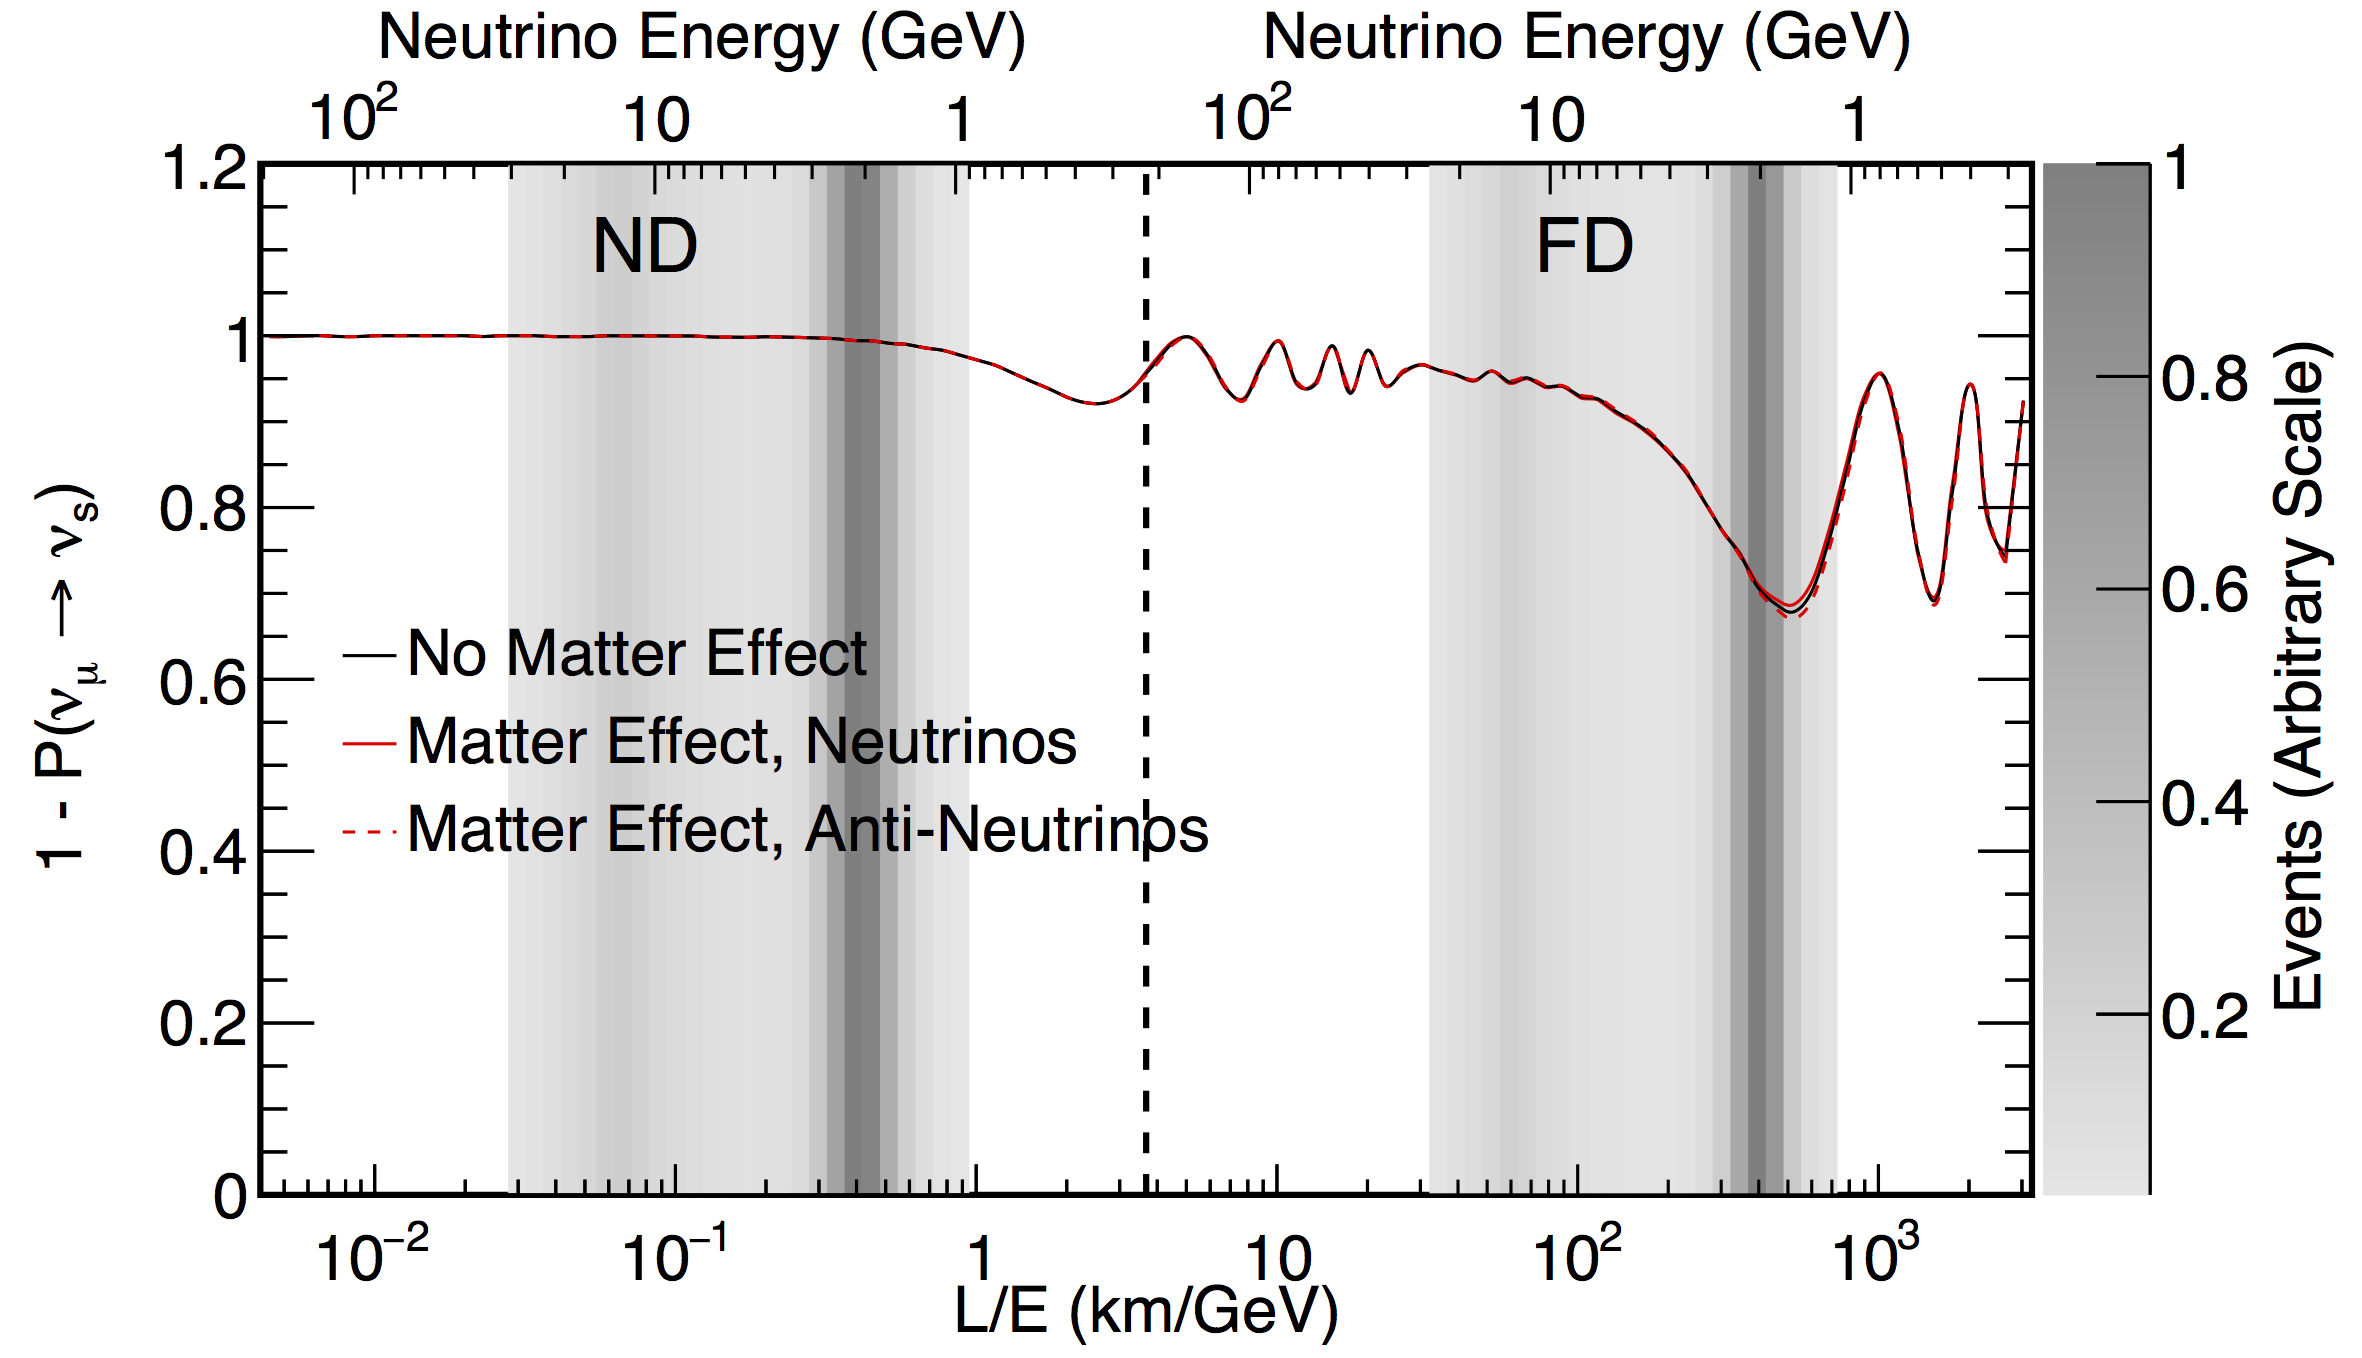
\includegraphics[width=0.95\textwidth]{figures/LOverE/LOverEPlotMatter.png} \\
    \\ \\
    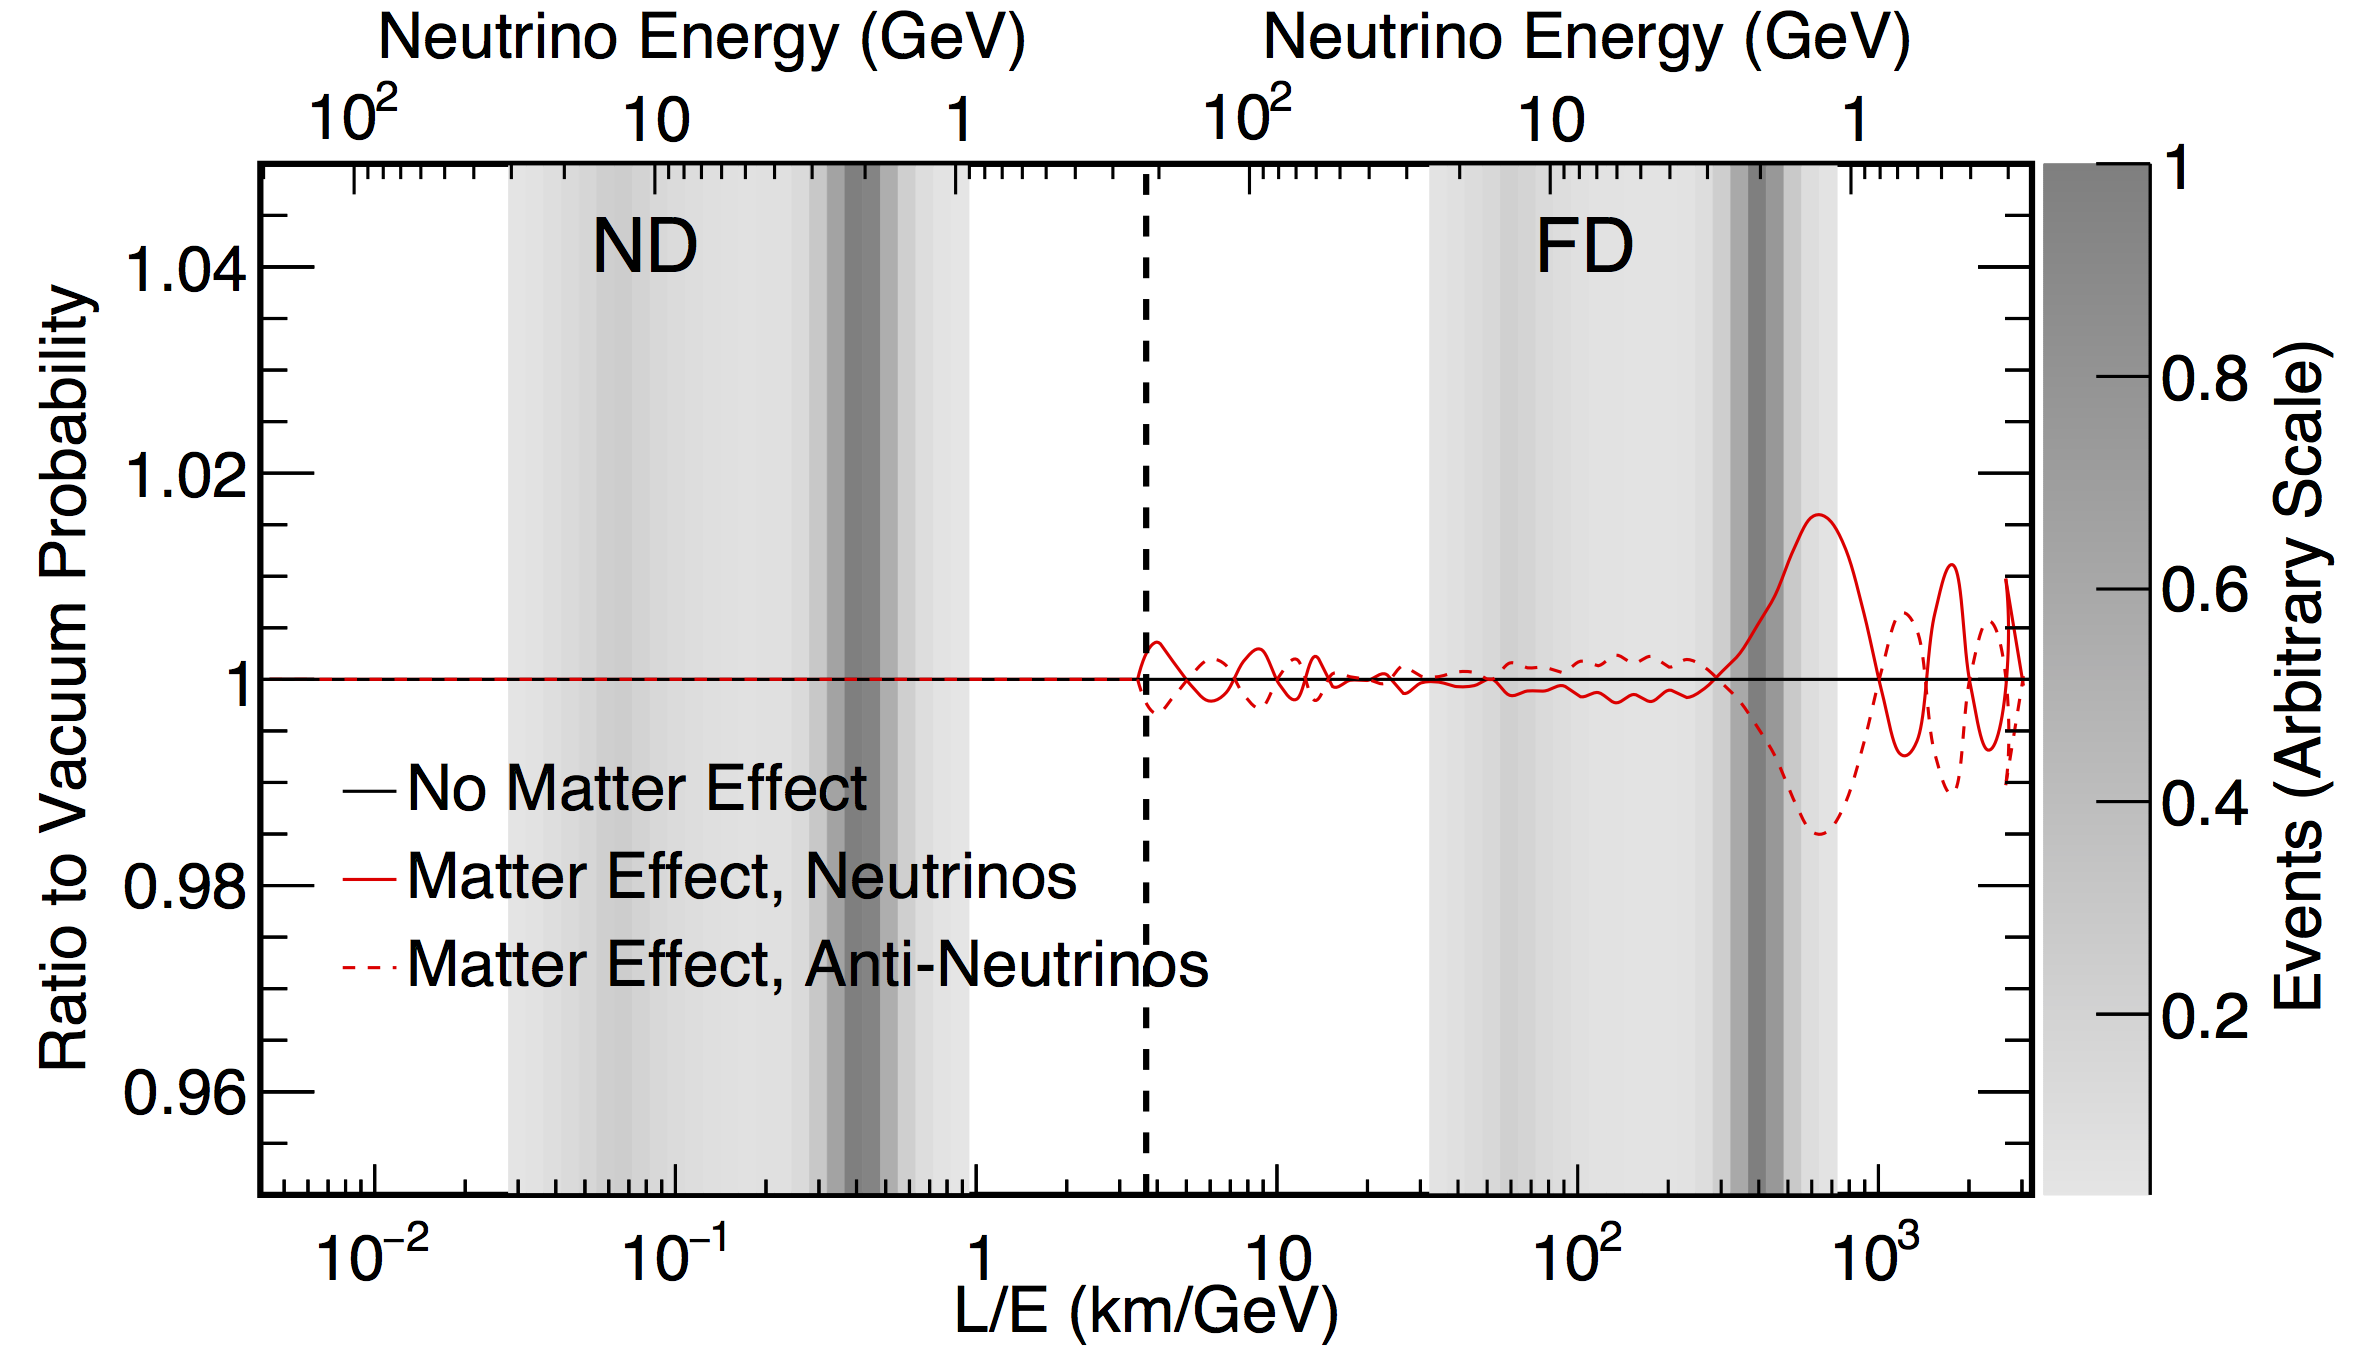
\includegraphics[width=0.95\textwidth]{figures/LOverE/LOverEPlotMatterRatio.png} \\
  \end{tabular}
  \caption[The Sterile Matter Effect]{Total active neutrino survival probability demonstrating the size of the sterile matter effect. The probabilities are shown in the top figure, the ratios of the matter affected probabilities to the vacuum probability is shown in the bottom figure. The black line shows the survival probability in vacuum. The solid (dashed) red line shows the survival probability for muon (anti-)neutrinos in matter. The grey bands show the neutrino energy spectra observed by \nova, with darker colors representing a higher intensity of neutrinos. Oscillation parameters are held fixed to values shown in table \ref{tab:LOverEValues}.}
  \label{fig:LOverEMatter}
\end{figure}

The maximum size of the effect is less than $2\%$ and occurs at about $1\unit{GeV}$. At the peak sensitivity region for the \nova~Far Detector, the effect is even smaller at about $1\%$. To contrast, the MSW effect for $\nue$ appearance effects the oscillation probabilities by $\sim 20\%$ in \nova~\cite{ref:ThesisEvan}. Nonetheless, the small sterile matter effect is included in the analysis presented here.
